%Chapter 4
\chapter{Results and validation}
\thispagestyle{empty}
\vspace{38em}
\hrulefill
\\

\enquote{\textit{It doesn't matter how beautiful your theory is, it doesn't matter how smart you are. If it doesn't agree with experiment, it's wrong.}} - Richard P. Feynman\\
\newpage
\section{Introduction}
This section will validate the simulation methodology through case studies. Mining compressed air systems were chosen as case studies based on the availability of data and the scope for energy and operational improvement. Two different mines were selected for the studies. 
\par 
Three case studies were performed. In case study 1 and 2, improvements were simulated on mine A and mine B respectively. In Case study three periodic simulation analysis is implemented using the simulation developed for case study 2. From the results of the case studies, the potential benefits compressed air simulations for the South Africa mining industry is estimated and discussed.

\section{Case study 1. Simulated improvements on mine A}
\subsection{System investigation}
Mine A represents a group of three gold mining shafts and a gold processing plant in the Free state province. The mine shafts and gold plant share a compressed network. Before this study, efforts had been made to optimise the system through \gls{dsm} energy projects. However, there may still be potential for further optimisation. An investigation was performed to gather data and understanding of the system and to identify potential energy and operation improvement strategies.
\par 
An air-flow distribution layout was developed for the system; a simplified layout is shown in \Cref{fig: Beatrix Air layout}. From the schematic along with information and data, an understanding of the air network’s operation was obtained. The system typically utilises 5 $MW$. During the drilling shift, the demand increases to 6 $MW$. \Cref{fig: Beatrix power baseline} shows the average weekday power profile between January and May 2016.

\begin{figure}[h!]
	\centering
	\fbox{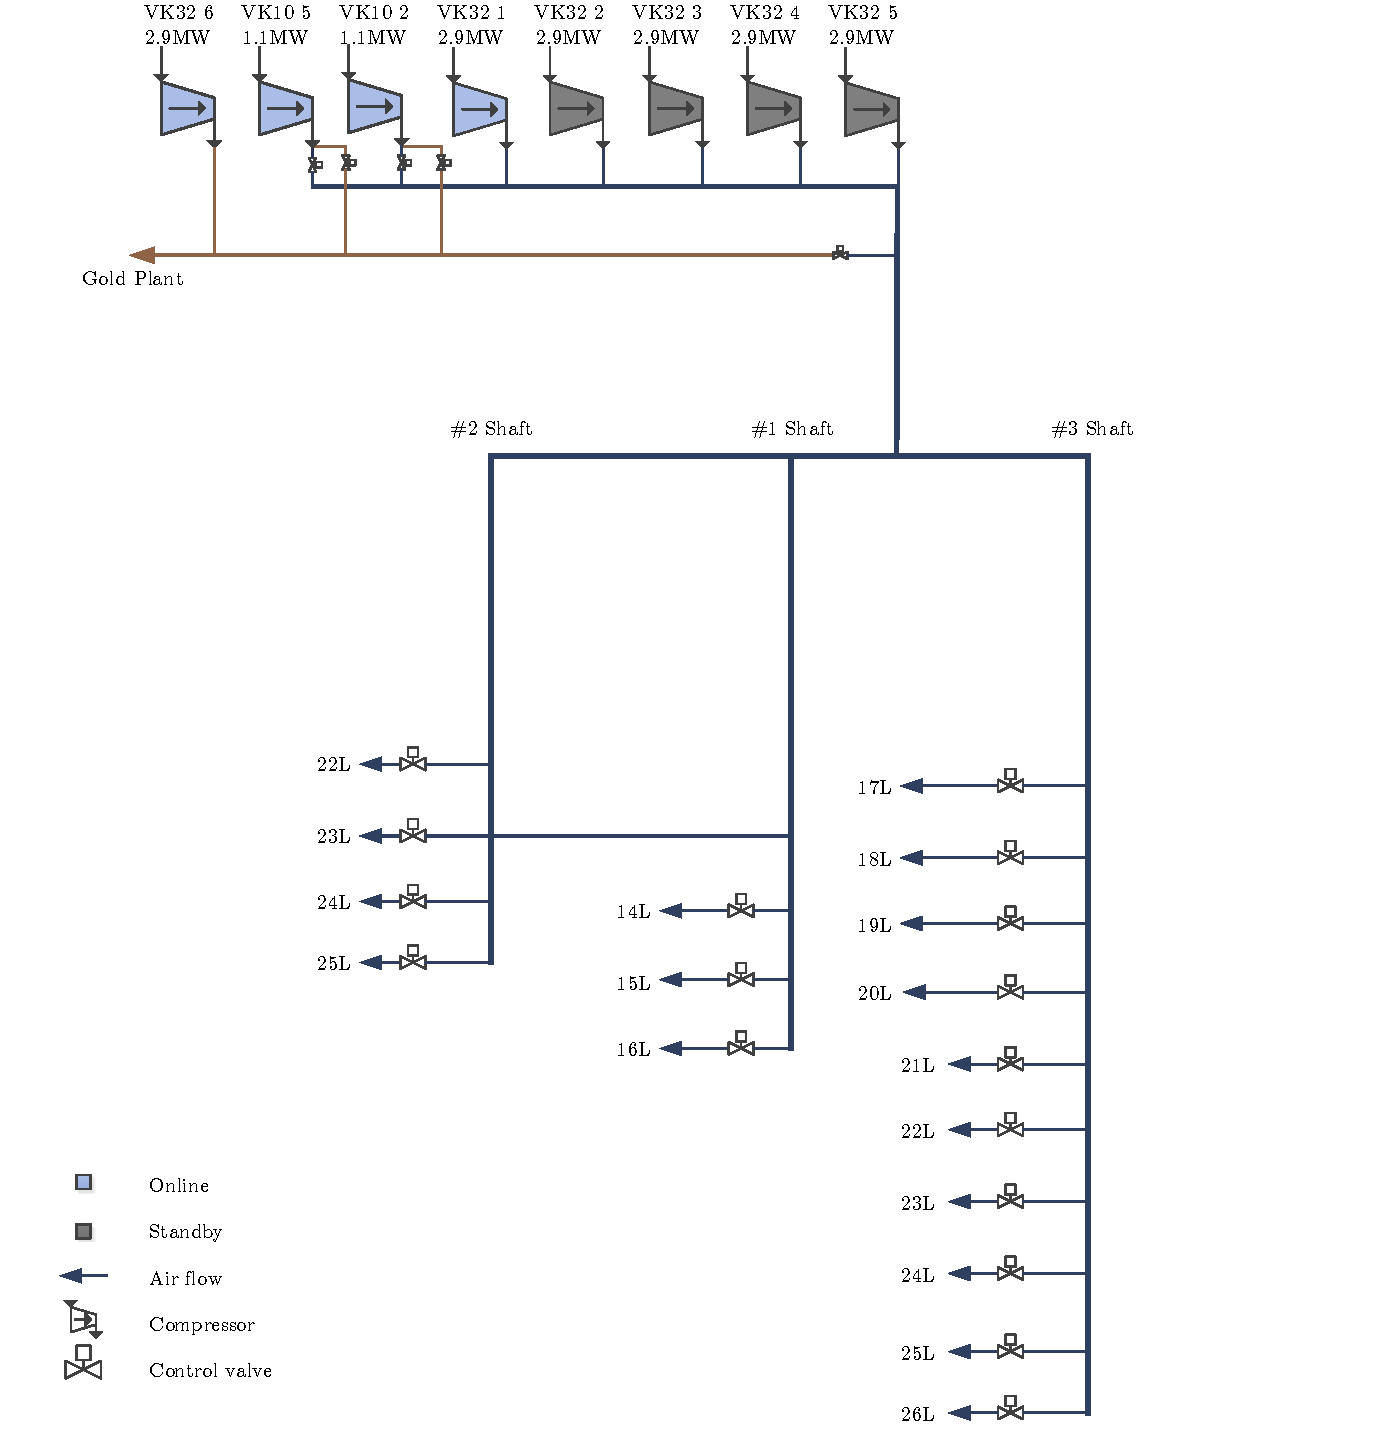
\includegraphics[trim =1cm -0.2cm 3.3cm -0.2cm,width=\textwidth]{Graphs/4/BeatLayout1/BeatLayout1.pdf}}
	\caption{Simplified process flow chart of the compressed air network}
	\label{fig: Beatrix Air layout}
\end{figure}
\clearpage
\begin{figure}[h!]
	\centering
	% GNUPLOT: LaTeX picture with Postscript
\begingroup
  \makeatletter
  \providecommand\color[2][]{%
    \GenericError{(gnuplot) \space\space\space\@spaces}{%
      Package color not loaded in conjunction with
      terminal option `colourtext'%
    }{See the gnuplot documentation for explanation.%
    }{Either use 'blacktext' in gnuplot or load the package
      color.sty in LaTeX.}%
    \renewcommand\color[2][]{}%
  }%
  \providecommand\includegraphics[2][]{%
    \GenericError{(gnuplot) \space\space\space\@spaces}{%
      Package graphicx or graphics not loaded%
    }{See the gnuplot documentation for explanation.%
    }{The gnuplot epslatex terminal needs graphicx.sty or graphics.sty.}%
    \renewcommand\includegraphics[2][]{}%
  }%
  \providecommand\rotatebox[2]{#2}%
  \@ifundefined{ifGPcolor}{%
    \newif\ifGPcolor
    \GPcolortrue
  }{}%
  \@ifundefined{ifGPblacktext}{%
    \newif\ifGPblacktext
    \GPblacktextfalse
  }{}%
  % define a \g@addto@macro without @ in the name:
  \let\gplgaddtomacro\g@addto@macro
  % define empty templates for all commands taking text:
  \gdef\gplbacktext{}%
  \gdef\gplfronttext{}%
  \makeatother
  \ifGPblacktext
    % no textcolor at all
    \def\colorrgb#1{}%
    \def\colorgray#1{}%
  \else
    % gray or color?
    \ifGPcolor
      \def\colorrgb#1{\color[rgb]{#1}}%
      \def\colorgray#1{\color[gray]{#1}}%
      \expandafter\def\csname LTw\endcsname{\color{white}}%
      \expandafter\def\csname LTb\endcsname{\color{black}}%
      \expandafter\def\csname LTa\endcsname{\color{black}}%
      \expandafter\def\csname LT0\endcsname{\color[rgb]{1,0,0}}%
      \expandafter\def\csname LT1\endcsname{\color[rgb]{0,1,0}}%
      \expandafter\def\csname LT2\endcsname{\color[rgb]{0,0,1}}%
      \expandafter\def\csname LT3\endcsname{\color[rgb]{1,0,1}}%
      \expandafter\def\csname LT4\endcsname{\color[rgb]{0,1,1}}%
      \expandafter\def\csname LT5\endcsname{\color[rgb]{1,1,0}}%
      \expandafter\def\csname LT6\endcsname{\color[rgb]{0,0,0}}%
      \expandafter\def\csname LT7\endcsname{\color[rgb]{1,0.3,0}}%
      \expandafter\def\csname LT8\endcsname{\color[rgb]{0.5,0.5,0.5}}%
    \else
      % gray
      \def\colorrgb#1{\color{black}}%
      \def\colorgray#1{\color[gray]{#1}}%
      \expandafter\def\csname LTw\endcsname{\color{white}}%
      \expandafter\def\csname LTb\endcsname{\color{black}}%
      \expandafter\def\csname LTa\endcsname{\color{black}}%
      \expandafter\def\csname LT0\endcsname{\color{black}}%
      \expandafter\def\csname LT1\endcsname{\color{black}}%
      \expandafter\def\csname LT2\endcsname{\color{black}}%
      \expandafter\def\csname LT3\endcsname{\color{black}}%
      \expandafter\def\csname LT4\endcsname{\color{black}}%
      \expandafter\def\csname LT5\endcsname{\color{black}}%
      \expandafter\def\csname LT6\endcsname{\color{black}}%
      \expandafter\def\csname LT7\endcsname{\color{black}}%
      \expandafter\def\csname LT8\endcsname{\color{black}}%
    \fi
  \fi
    \setlength{\unitlength}{0.0500bp}%
    \ifx\gptboxheight\undefined%
      \newlength{\gptboxheight}%
      \newlength{\gptboxwidth}%
      \newsavebox{\gptboxtext}%
    \fi%
    \setlength{\fboxrule}{0.5pt}%
    \setlength{\fboxsep}{1pt}%
\begin{picture}(9360.00,3024.00)%
    \gplgaddtomacro\gplbacktext{%
      \colorrgb{0.00,0.00,0.00}%
      \put(550,704){\makebox(0,0)[r]{\strut{}$0$}}%
      \colorrgb{0.00,0.00,0.00}%
      \put(550,1047){\makebox(0,0)[r]{\strut{}$1$}}%
      \colorrgb{0.00,0.00,0.00}%
      \put(550,1389){\makebox(0,0)[r]{\strut{}$2$}}%
      \colorrgb{0.00,0.00,0.00}%
      \put(550,1732){\makebox(0,0)[r]{\strut{}$3$}}%
      \colorrgb{0.00,0.00,0.00}%
      \put(550,2074){\makebox(0,0)[r]{\strut{}$4$}}%
      \colorrgb{0.00,0.00,0.00}%
      \put(550,2417){\makebox(0,0)[r]{\strut{}$5$}}%
      \colorrgb{0.00,0.00,0.00}%
      \put(550,2759){\makebox(0,0)[r]{\strut{}$6$}}%
      \colorrgb{0.00,0.00,0.00}%
      \put(682,484){\makebox(0,0){\strut{}00:00}}%
      \colorrgb{0.00,0.00,0.00}%
      \put(2062,484){\makebox(0,0){\strut{}04:00}}%
      \colorrgb{0.00,0.00,0.00}%
      \put(3442,484){\makebox(0,0){\strut{}08:00}}%
      \colorrgb{0.00,0.00,0.00}%
      \put(4822,484){\makebox(0,0){\strut{}12:00}}%
      \colorrgb{0.00,0.00,0.00}%
      \put(6202,484){\makebox(0,0){\strut{}16:00}}%
      \colorrgb{0.00,0.00,0.00}%
      \put(7582,484){\makebox(0,0){\strut{}20:00}}%
      \colorrgb{0.00,0.00,0.00}%
      \put(8962,484){\makebox(0,0){\strut{}00:00}}%
    }%
    \gplgaddtomacro\gplfronttext{%
      \csname LTb\endcsname%
      \put(176,1731){\rotatebox{-270}{\makebox(0,0){\strut{}Power $(MW)$}}}%
      \put(4822,154){\makebox(0,0){\strut{}Time of Day}}%
    }%
    \gplbacktext
    \put(0,0){\fbox{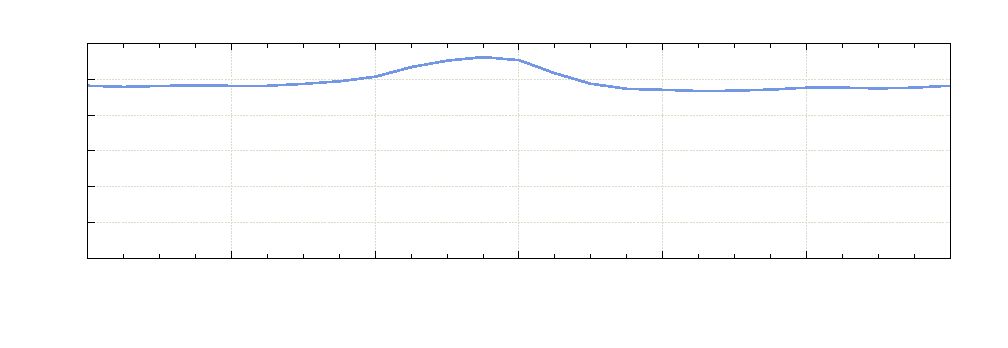
\includegraphics[trim=0 0 0.1cm 0, clip]{Graphs/4/BeetBaseline/Power/Power}}}%
    \gplfronttext
  \end{picture}%
\endgroup

	\caption{Average power profile}
	\label{fig: Beatrix power baseline}
\end{figure}

\par 
 Seven compresses are available in the system. Five large compressors (VK32) rated at 2.9 $MW$ each and two smaller compressors (VK10) with a power rating of 1.1 $MW$ each. No more than four compressors are required at any time; the other compressors are therefore on standby. Air is supplied to the sections in three mining shafts as well as a gold processing plant on the surface. 
 \par 
 The mine normally operates the compressors with a constant pressure setpoint of 500 \glssymbol{kpa}. The setpoint is kept high for the gold processing plant, which requires constant high pressure throughout the day. This constraint makes it difficult to reduce the setpoints of the compressor. It is possible to control the air supply pressure to the gold plant independently from the rest of the network. The supply to the gold plant by controlled by the surface valves.
 \par 
 The evening Eskom energy peak time was identified as a period where savings could be obtained. During this time, air is not required underground as blasting is scheduled. Due to the energy tariff structure, interventions during the energy peak also maximise the financial benefit for the mine. Compressor setpoint control and underground valve control were identified as strategies to achieve these savings. Due to the risk of loss of production, the mine would not allow practically testing the scenario on the actual system. The simulation was therefore required to accurately calculate and analyse the benefits of the of compressor set points. A model was developed to test these scenarios.

\subsection{Model development}
With the data and understanding gathered from the investigation, a model was developed using the \gls{ptb} software tool and the methodology discussed in Chapter 3. First, the simulation boundary was selected to include the measured flows to each level underground, as well as the surface processing plant. For highest accuracy, the simulation step size was set to 30 minutes to match the available data resolution.
\par
The simulation component models were developed and calibrated using the respective methods discussed in chapter 3. The following assumptions were made to simplify the model development:
\begin{itemize}
	\item The effect of compressed air after-cooling is negligible
	\item Heat transfer over the pipe length is negligible
	\item Underground temperature and humidity remained constant for each level
	\item Surface ambient air conditions followed normal summer trend
\end{itemize} 
The model components were calibrated so that the simulated outputs matched data from the real system. The process flow diagram for the simulation is shown in \Cref{fig: BEET Baseline model}. The model data inputs and outputs are described in \Cref{table: Mine A inputs/outputs}.

\begin{table}[h!]
	\centering
	\begin{tabular}{ll}
		\hline
		Inputs \hspace*{4cm} &Outputs \hspace*{4cm} \\ \hline
		Level measured flows&Compressor powers \\
		Compressor schedules& Network flows \\
		Compressor setpoints& Network pressures \\
		Underground valve setpoints& \\
		\hline
	\end{tabular}
	\caption{Data inputs and outputs for the Case study 1 simulation model }
	\label{table: Mine A inputs/outputs}
\end{table}


\subsection{Verification of model}
Verification was performed to ensure that simulated output accuracy was $>95$\%. \Cref{fig: Verification power Beatrix}, \Cref{fig: Verification power Beatrix} and \Cref{fig: Verification Pressure Beatrix} show the to total simulated power, flow and outlet pressure of the compressors compared to the system. The average accuracy for the power and total flow was 97.34\% and 97.01\% respectively. Both these parameters were well within the target relative error of 5\% relative error. The accuracy of the outlet pressure was 99.1\%. 

 \begin{table}[h!]
	\label{Beet verification table}
	\centering
	\begin{tabular}{p{0.5cm}p{8cm}p{5cm}r}
		\hline
		&Verification method & Result & $Err_{\%}$\\
		\hhline{====}
		\\ \multicolumn{4}{l}{\textbf{ Total Flow}}\\
		&Residual Difference  & 0.25 kg/s & 2.73\% \\
		&\gls{mae} 					 & 0.27 kg/s error & 3.0\% \\
		&Coefficient of determination & $r^2 =0.99$ & -\\ 
		\\ \multicolumn{4}{l}{\textbf{ Total power}}\\
		&Residual Difference  & 0.02 MW & 0.57\% \\
		&\gls{mae} 					 & 0.14 MW error & 2.78\% \\
		 &Coefficient of determination & $r^2 =0.91$ & -\\ 
		\\ \multicolumn{4}{l}{\textbf{ Compressor outlet pressure}}\\
		&Residual Difference  &0.03 kPa & 0.01\% \\
		&\gls{mae} 					 & 0.21 kPa error & 0.03\% \\
		&Coefficient of determination & $r^2 =0.99$ & -\\
	\\ 	\hline
	\end{tabular} 
	\caption{Case study 1: Verification of simulation model}
\end{table}
\begin{figure}[h!]
	\centering
	% GNUPLOT: LaTeX picture with Postscript
\begingroup
  \makeatletter
  \providecommand\color[2][]{%
    \GenericError{(gnuplot) \space\space\space\@spaces}{%
      Package color not loaded in conjunction with
      terminal option `colourtext'%
    }{See the gnuplot documentation for explanation.%
    }{Either use 'blacktext' in gnuplot or load the package
      color.sty in LaTeX.}%
    \renewcommand\color[2][]{}%
  }%
  \providecommand\includegraphics[2][]{%
    \GenericError{(gnuplot) \space\space\space\@spaces}{%
      Package graphicx or graphics not loaded%
    }{See the gnuplot documentation for explanation.%
    }{The gnuplot epslatex terminal needs graphicx.sty or graphics.sty.}%
    \renewcommand\includegraphics[2][]{}%
  }%
  \providecommand\rotatebox[2]{#2}%
  \@ifundefined{ifGPcolor}{%
    \newif\ifGPcolor
    \GPcolortrue
  }{}%
  \@ifundefined{ifGPblacktext}{%
    \newif\ifGPblacktext
    \GPblacktextfalse
  }{}%
  % define a \g@addto@macro without @ in the name:
  \let\gplgaddtomacro\g@addto@macro
  % define empty templates for all commands taking text:
  \gdef\gplbacktext{}%
  \gdef\gplfronttext{}%
  \makeatother
  \ifGPblacktext
    % no textcolor at all
    \def\colorrgb#1{}%
    \def\colorgray#1{}%
  \else
    % gray or color?
    \ifGPcolor
      \def\colorrgb#1{\color[rgb]{#1}}%
      \def\colorgray#1{\color[gray]{#1}}%
      \expandafter\def\csname LTw\endcsname{\color{white}}%
      \expandafter\def\csname LTb\endcsname{\color{black}}%
      \expandafter\def\csname LTa\endcsname{\color{black}}%
      \expandafter\def\csname LT0\endcsname{\color[rgb]{1,0,0}}%
      \expandafter\def\csname LT1\endcsname{\color[rgb]{0,1,0}}%
      \expandafter\def\csname LT2\endcsname{\color[rgb]{0,0,1}}%
      \expandafter\def\csname LT3\endcsname{\color[rgb]{1,0,1}}%
      \expandafter\def\csname LT4\endcsname{\color[rgb]{0,1,1}}%
      \expandafter\def\csname LT5\endcsname{\color[rgb]{1,1,0}}%
      \expandafter\def\csname LT6\endcsname{\color[rgb]{0,0,0}}%
      \expandafter\def\csname LT7\endcsname{\color[rgb]{1,0.3,0}}%
      \expandafter\def\csname LT8\endcsname{\color[rgb]{0.5,0.5,0.5}}%
    \else
      % gray
      \def\colorrgb#1{\color{black}}%
      \def\colorgray#1{\color[gray]{#1}}%
      \expandafter\def\csname LTw\endcsname{\color{white}}%
      \expandafter\def\csname LTb\endcsname{\color{black}}%
      \expandafter\def\csname LTa\endcsname{\color{black}}%
      \expandafter\def\csname LT0\endcsname{\color{black}}%
      \expandafter\def\csname LT1\endcsname{\color{black}}%
      \expandafter\def\csname LT2\endcsname{\color{black}}%
      \expandafter\def\csname LT3\endcsname{\color{black}}%
      \expandafter\def\csname LT4\endcsname{\color{black}}%
      \expandafter\def\csname LT5\endcsname{\color{black}}%
      \expandafter\def\csname LT6\endcsname{\color{black}}%
      \expandafter\def\csname LT7\endcsname{\color{black}}%
      \expandafter\def\csname LT8\endcsname{\color{black}}%
    \fi
  \fi
    \setlength{\unitlength}{0.0500bp}%
    \ifx\gptboxheight\undefined%
      \newlength{\gptboxheight}%
      \newlength{\gptboxwidth}%
      \newsavebox{\gptboxtext}%
    \fi%
    \setlength{\fboxrule}{0.5pt}%
    \setlength{\fboxsep}{1pt}%
\begin{picture}(9360.00,4032.00)%
    \gplgaddtomacro\gplbacktext{%
      \colorrgb{0.00,0.00,0.00}%
      \put(550,924){\makebox(0,0)[r]{\strut{}$0$}}%
      \colorrgb{0.00,0.00,0.00}%
      \put(550,1279){\makebox(0,0)[r]{\strut{}$1$}}%
      \colorrgb{0.00,0.00,0.00}%
      \put(550,1635){\makebox(0,0)[r]{\strut{}$2$}}%
      \colorrgb{0.00,0.00,0.00}%
      \put(550,1990){\makebox(0,0)[r]{\strut{}$3$}}%
      \colorrgb{0.00,0.00,0.00}%
      \put(550,2346){\makebox(0,0)[r]{\strut{}$4$}}%
      \colorrgb{0.00,0.00,0.00}%
      \put(550,2701){\makebox(0,0)[r]{\strut{}$5$}}%
      \colorrgb{0.00,0.00,0.00}%
      \put(550,3056){\makebox(0,0)[r]{\strut{}$6$}}%
      \colorrgb{0.00,0.00,0.00}%
      \put(550,3412){\makebox(0,0)[r]{\strut{}$7$}}%
      \colorrgb{0.00,0.00,0.00}%
      \put(550,3767){\makebox(0,0)[r]{\strut{}$8$}}%
      \colorrgb{0.00,0.00,0.00}%
      \put(682,704){\makebox(0,0){\strut{}00:00}}%
      \colorrgb{0.00,0.00,0.00}%
      \put(1937,704){\makebox(0,0){\strut{}04:00}}%
      \colorrgb{0.00,0.00,0.00}%
      \put(3193,704){\makebox(0,0){\strut{}08:00}}%
      \colorrgb{0.00,0.00,0.00}%
      \put(4448,704){\makebox(0,0){\strut{}12:00}}%
      \colorrgb{0.00,0.00,0.00}%
      \put(5703,704){\makebox(0,0){\strut{}16:00}}%
      \colorrgb{0.00,0.00,0.00}%
      \put(6959,704){\makebox(0,0){\strut{}20:00}}%
      \colorrgb{0.00,0.00,0.00}%
      \put(8214,704){\makebox(0,0){\strut{}00:00}}%
      \colorrgb{0.00,0.00,0.00}%
      \put(8346,924){\makebox(0,0)[l]{\strut{}$0$}}%
      \colorrgb{0.00,0.00,0.00}%
      \put(8346,2061){\makebox(0,0)[l]{\strut{}$10$}}%
      \colorrgb{0.00,0.00,0.00}%
      \put(8346,3198){\makebox(0,0)[l]{\strut{}$20$}}%
    }%
    \gplgaddtomacro\gplfronttext{%
      \csname LTb\endcsname%
      \put(176,2345){\rotatebox{-270}{\makebox(0,0){\strut{}Power $(MW)$}}}%
      \put(8851,2345){\rotatebox{-270}{\makebox(0,0){\strut{}$\%$ $error$}}}%
      \put(4448,374){\makebox(0,0){\strut{}Time of use}}%
      \csname LTb\endcsname%
      \put(2175,173){\makebox(0,0)[r]{\strut{}Baseline power}}%
      \csname LTb\endcsname%
      \put(5010,173){\makebox(0,0)[r]{\strut{}Simulated power}}%
      \csname LTb\endcsname%
      \put(7700,173){\makebox(0,0)[r]{\strut{}Rel. Error}}%
    }%
    \gplbacktext
    \put(0,0){\fbox{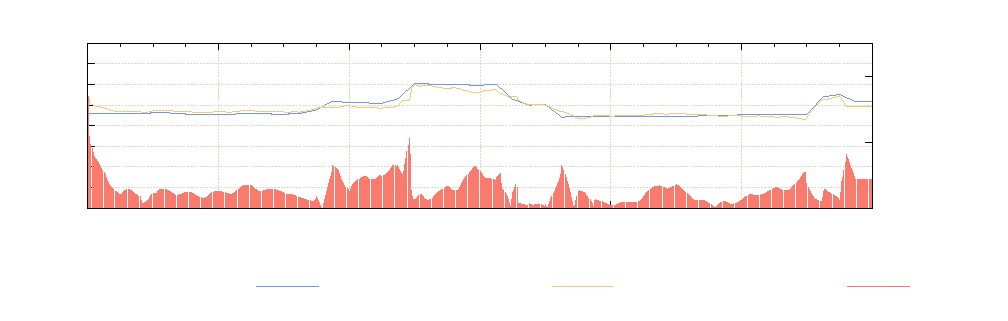
\includegraphics[trim=0 0 0.1cm 0, clip]{Graphs/4/BeetVerify/Power/Power}}}%
    \gplfronttext
  \end{picture}%
\endgroup

	\caption{The simulated power compared to the actual measurement}
	\label{fig: Verification power Beatrix}
\end{figure}
\begin{figure}[h!]
	\centering
	% GNUPLOT: LaTeX picture with Postscript
\begingroup
  \makeatletter
  \providecommand\color[2][]{%
    \GenericError{(gnuplot) \space\space\space\@spaces}{%
      Package color not loaded in conjunction with
      terminal option `colourtext'%
    }{See the gnuplot documentation for explanation.%
    }{Either use 'blacktext' in gnuplot or load the package
      color.sty in LaTeX.}%
    \renewcommand\color[2][]{}%
  }%
  \providecommand\includegraphics[2][]{%
    \GenericError{(gnuplot) \space\space\space\@spaces}{%
      Package graphicx or graphics not loaded%
    }{See the gnuplot documentation for explanation.%
    }{The gnuplot epslatex terminal needs graphicx.sty or graphics.sty.}%
    \renewcommand\includegraphics[2][]{}%
  }%
  \providecommand\rotatebox[2]{#2}%
  \@ifundefined{ifGPcolor}{%
    \newif\ifGPcolor
    \GPcolortrue
  }{}%
  \@ifundefined{ifGPblacktext}{%
    \newif\ifGPblacktext
    \GPblacktextfalse
  }{}%
  % define a \g@addto@macro without @ in the name:
  \let\gplgaddtomacro\g@addto@macro
  % define empty templates for all commands taking text:
  \gdef\gplbacktext{}%
  \gdef\gplfronttext{}%
  \makeatother
  \ifGPblacktext
    % no textcolor at all
    \def\colorrgb#1{}%
    \def\colorgray#1{}%
  \else
    % gray or color?
    \ifGPcolor
      \def\colorrgb#1{\color[rgb]{#1}}%
      \def\colorgray#1{\color[gray]{#1}}%
      \expandafter\def\csname LTw\endcsname{\color{white}}%
      \expandafter\def\csname LTb\endcsname{\color{black}}%
      \expandafter\def\csname LTa\endcsname{\color{black}}%
      \expandafter\def\csname LT0\endcsname{\color[rgb]{1,0,0}}%
      \expandafter\def\csname LT1\endcsname{\color[rgb]{0,1,0}}%
      \expandafter\def\csname LT2\endcsname{\color[rgb]{0,0,1}}%
      \expandafter\def\csname LT3\endcsname{\color[rgb]{1,0,1}}%
      \expandafter\def\csname LT4\endcsname{\color[rgb]{0,1,1}}%
      \expandafter\def\csname LT5\endcsname{\color[rgb]{1,1,0}}%
      \expandafter\def\csname LT6\endcsname{\color[rgb]{0,0,0}}%
      \expandafter\def\csname LT7\endcsname{\color[rgb]{1,0.3,0}}%
      \expandafter\def\csname LT8\endcsname{\color[rgb]{0.5,0.5,0.5}}%
    \else
      % gray
      \def\colorrgb#1{\color{black}}%
      \def\colorgray#1{\color[gray]{#1}}%
      \expandafter\def\csname LTw\endcsname{\color{white}}%
      \expandafter\def\csname LTb\endcsname{\color{black}}%
      \expandafter\def\csname LTa\endcsname{\color{black}}%
      \expandafter\def\csname LT0\endcsname{\color{black}}%
      \expandafter\def\csname LT1\endcsname{\color{black}}%
      \expandafter\def\csname LT2\endcsname{\color{black}}%
      \expandafter\def\csname LT3\endcsname{\color{black}}%
      \expandafter\def\csname LT4\endcsname{\color{black}}%
      \expandafter\def\csname LT5\endcsname{\color{black}}%
      \expandafter\def\csname LT6\endcsname{\color{black}}%
      \expandafter\def\csname LT7\endcsname{\color{black}}%
      \expandafter\def\csname LT8\endcsname{\color{black}}%
    \fi
  \fi
    \setlength{\unitlength}{0.0500bp}%
    \ifx\gptboxheight\undefined%
      \newlength{\gptboxheight}%
      \newlength{\gptboxwidth}%
      \newsavebox{\gptboxtext}%
    \fi%
    \setlength{\fboxrule}{0.5pt}%
    \setlength{\fboxsep}{1pt}%
\begin{picture}(9360.00,4032.00)%
    \gplgaddtomacro\gplbacktext{%
      \colorrgb{0.00,0.00,0.00}%
      \put(682,924){\makebox(0,0)[r]{\strut{}$0$}}%
      \colorrgb{0.00,0.00,0.00}%
      \put(682,1872){\makebox(0,0)[r]{\strut{}$5$}}%
      \colorrgb{0.00,0.00,0.00}%
      \put(682,2819){\makebox(0,0)[r]{\strut{}$10$}}%
      \colorrgb{0.00,0.00,0.00}%
      \put(682,3767){\makebox(0,0)[r]{\strut{}$15$}}%
      \colorrgb{0.00,0.00,0.00}%
      \put(814,704){\makebox(0,0){\strut{}00:00}}%
      \colorrgb{0.00,0.00,0.00}%
      \put(2047,704){\makebox(0,0){\strut{}04:00}}%
      \colorrgb{0.00,0.00,0.00}%
      \put(3281,704){\makebox(0,0){\strut{}08:00}}%
      \colorrgb{0.00,0.00,0.00}%
      \put(4514,704){\makebox(0,0){\strut{}12:00}}%
      \colorrgb{0.00,0.00,0.00}%
      \put(5747,704){\makebox(0,0){\strut{}16:00}}%
      \colorrgb{0.00,0.00,0.00}%
      \put(6981,704){\makebox(0,0){\strut{}20:00}}%
      \colorrgb{0.00,0.00,0.00}%
      \put(8214,704){\makebox(0,0){\strut{}00:00}}%
      \colorrgb{0.00,0.00,0.00}%
      \put(8346,924){\makebox(0,0)[l]{\strut{}$0$}}%
      \colorrgb{0.00,0.00,0.00}%
      \put(8346,2061){\makebox(0,0)[l]{\strut{}$10$}}%
      \colorrgb{0.00,0.00,0.00}%
      \put(8346,3198){\makebox(0,0)[l]{\strut{}$20$}}%
    }%
    \gplgaddtomacro\gplfronttext{%
      \csname LTb\endcsname%
      \put(176,2345){\rotatebox{-270}{\makebox(0,0){\strut{}Flow $(kg/s)$}}}%
      \put(8851,2345){\rotatebox{-270}{\makebox(0,0){\strut{}$\% error$}}}%
      \put(4514,374){\makebox(0,0){\strut{}Time of Day}}%
      \csname LTb\endcsname%
      \put(2307,173){\makebox(0,0)[r]{\strut{}Baseline flow}}%
      \csname LTb\endcsname%
      \put(5010,173){\makebox(0,0)[r]{\strut{}Simulated flow}}%
      \csname LTb\endcsname%
      \put(7713,173){\makebox(0,0)[r]{\strut{}Error}}%
    }%
    \gplbacktext
    \put(0,0){\fbox{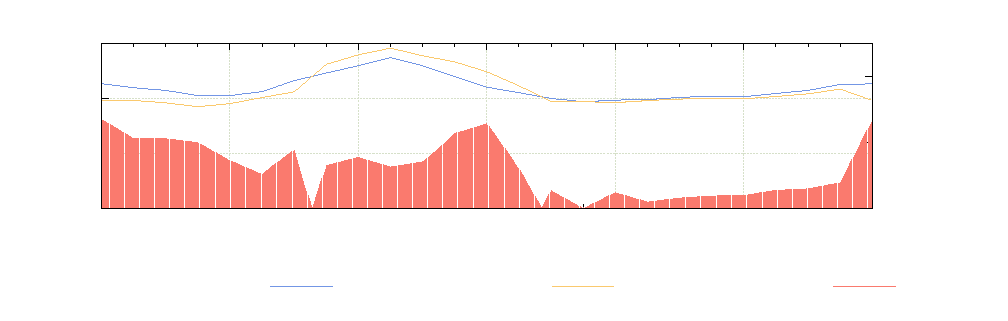
\includegraphics[trim=0 0 0.1cm 0, clip]{Graphs/4/BeetVerify/Flow/Flow}}}%
    \gplfronttext
  \end{picture}%
\endgroup

	\caption{The simulated flow compared to the actual measurement}
	\label{fig: Verification flow Beatrix}
\end{figure}
\begin{figure}[h!]
	\centering
	% GNUPLOT: LaTeX picture with Postscript
\begingroup
  \makeatletter
  \providecommand\color[2][]{%
    \GenericError{(gnuplot) \space\space\space\@spaces}{%
      Package color not loaded in conjunction with
      terminal option `colourtext'%
    }{See the gnuplot documentation for explanation.%
    }{Either use 'blacktext' in gnuplot or load the package
      color.sty in LaTeX.}%
    \renewcommand\color[2][]{}%
  }%
  \providecommand\includegraphics[2][]{%
    \GenericError{(gnuplot) \space\space\space\@spaces}{%
      Package graphicx or graphics not loaded%
    }{See the gnuplot documentation for explanation.%
    }{The gnuplot epslatex terminal needs graphicx.sty or graphics.sty.}%
    \renewcommand\includegraphics[2][]{}%
  }%
  \providecommand\rotatebox[2]{#2}%
  \@ifundefined{ifGPcolor}{%
    \newif\ifGPcolor
    \GPcolortrue
  }{}%
  \@ifundefined{ifGPblacktext}{%
    \newif\ifGPblacktext
    \GPblacktextfalse
  }{}%
  % define a \g@addto@macro without @ in the name:
  \let\gplgaddtomacro\g@addto@macro
  % define empty templates for all commands taking text:
  \gdef\gplbacktext{}%
  \gdef\gplfronttext{}%
  \makeatother
  \ifGPblacktext
    % no textcolor at all
    \def\colorrgb#1{}%
    \def\colorgray#1{}%
  \else
    % gray or color?
    \ifGPcolor
      \def\colorrgb#1{\color[rgb]{#1}}%
      \def\colorgray#1{\color[gray]{#1}}%
      \expandafter\def\csname LTw\endcsname{\color{white}}%
      \expandafter\def\csname LTb\endcsname{\color{black}}%
      \expandafter\def\csname LTa\endcsname{\color{black}}%
      \expandafter\def\csname LT0\endcsname{\color[rgb]{1,0,0}}%
      \expandafter\def\csname LT1\endcsname{\color[rgb]{0,1,0}}%
      \expandafter\def\csname LT2\endcsname{\color[rgb]{0,0,1}}%
      \expandafter\def\csname LT3\endcsname{\color[rgb]{1,0,1}}%
      \expandafter\def\csname LT4\endcsname{\color[rgb]{0,1,1}}%
      \expandafter\def\csname LT5\endcsname{\color[rgb]{1,1,0}}%
      \expandafter\def\csname LT6\endcsname{\color[rgb]{0,0,0}}%
      \expandafter\def\csname LT7\endcsname{\color[rgb]{1,0.3,0}}%
      \expandafter\def\csname LT8\endcsname{\color[rgb]{0.5,0.5,0.5}}%
    \else
      % gray
      \def\colorrgb#1{\color{black}}%
      \def\colorgray#1{\color[gray]{#1}}%
      \expandafter\def\csname LTw\endcsname{\color{white}}%
      \expandafter\def\csname LTb\endcsname{\color{black}}%
      \expandafter\def\csname LTa\endcsname{\color{black}}%
      \expandafter\def\csname LT0\endcsname{\color{black}}%
      \expandafter\def\csname LT1\endcsname{\color{black}}%
      \expandafter\def\csname LT2\endcsname{\color{black}}%
      \expandafter\def\csname LT3\endcsname{\color{black}}%
      \expandafter\def\csname LT4\endcsname{\color{black}}%
      \expandafter\def\csname LT5\endcsname{\color{black}}%
      \expandafter\def\csname LT6\endcsname{\color{black}}%
      \expandafter\def\csname LT7\endcsname{\color{black}}%
      \expandafter\def\csname LT8\endcsname{\color{black}}%
    \fi
  \fi
    \setlength{\unitlength}{0.0500bp}%
    \ifx\gptboxheight\undefined%
      \newlength{\gptboxheight}%
      \newlength{\gptboxwidth}%
      \newsavebox{\gptboxtext}%
    \fi%
    \setlength{\fboxrule}{0.5pt}%
    \setlength{\fboxsep}{1pt}%
\begin{picture}(9360.00,2772.00)%
    \gplgaddtomacro\gplbacktext{%
      \colorrgb{0.00,0.00,0.00}%
      \put(814,924){\makebox(0,0)[r]{\strut{}$300$}}%
      \colorrgb{0.00,0.00,0.00}%
      \put(814,1452){\makebox(0,0)[r]{\strut{}$350$}}%
      \colorrgb{0.00,0.00,0.00}%
      \put(814,1979){\makebox(0,0)[r]{\strut{}$400$}}%
      \colorrgb{0.00,0.00,0.00}%
      \put(814,2507){\makebox(0,0)[r]{\strut{}$450$}}%
      \colorrgb{0.00,0.00,0.00}%
      \put(946,704){\makebox(0,0){\strut{}00:00}}%
      \colorrgb{0.00,0.00,0.00}%
      \put(2157,704){\makebox(0,0){\strut{}04:00}}%
      \colorrgb{0.00,0.00,0.00}%
      \put(3369,704){\makebox(0,0){\strut{}08:00}}%
      \colorrgb{0.00,0.00,0.00}%
      \put(4580,704){\makebox(0,0){\strut{}12:00}}%
      \colorrgb{0.00,0.00,0.00}%
      \put(5791,704){\makebox(0,0){\strut{}16:00}}%
      \colorrgb{0.00,0.00,0.00}%
      \put(7003,704){\makebox(0,0){\strut{}20:00}}%
      \colorrgb{0.00,0.00,0.00}%
      \put(8214,704){\makebox(0,0){\strut{}00:00}}%
      \colorrgb{0.00,0.00,0.00}%
      \put(8346,924){\makebox(0,0)[l]{\strut{}$0$}}%
      \colorrgb{0.00,0.00,0.00}%
      \put(8346,1557){\makebox(0,0)[l]{\strut{}$10$}}%
      \colorrgb{0.00,0.00,0.00}%
      \put(8346,2190){\makebox(0,0)[l]{\strut{}$20$}}%
    }%
    \gplgaddtomacro\gplfronttext{%
      \csname LTb\endcsname%
      \put(176,1715){\rotatebox{-270}{\makebox(0,0){\strut{}Pressure $(kPa)$}}}%
      \put(8851,1715){\rotatebox{-270}{\makebox(0,0){\strut{}$\% error$}}}%
      \put(4580,374){\makebox(0,0){\strut{}Time of Day}}%
      \csname LTb\endcsname%
      \put(2241,173){\makebox(0,0)[r]{\strut{}Baseline press.}}%
      \csname LTb\endcsname%
      \put(5208,173){\makebox(0,0)[r]{\strut{}Simulated press.}}%
      \csname LTb\endcsname%
      \put(8175,173){\makebox(0,0)[r]{\strut{}Error}}%
    }%
    \gplbacktext
    \put(0,0){
\includegraphics{Graphs/4/BeetVerify/Pressure/Pressure}}%
    \gplfronttext
  \end{picture}%
\endgroup

	\caption{The simulated pressure compared to the actual measurement}
	\label{fig: Verification Pressure Beatrix}
\end{figure}
\par
The accuracy of the model was checked in more detail to ensure that each modelled parameter matched the actual measurement with high accuracy. \Cref{Table: A verification} shows the precision each measured simulation output in the model.
\subsection{Execute simulations}
\subsubsection{Scenario 1. Compressor set points}
The Eskom evening peak tariff time occurs during the blasting shift. During this time, the pressure requirements underground are lower than the rest of the day. Reducing pressure in the network reduces power as less work is required from the compressors. Additionally, losses caused by air leaks are reduced. However, lowering the pressure setpoint of the compressors requires independently controlling the air to the gold plant. 
\par 
The compressor set-points were reduced for the simulation model to 420 \glssymbol{kpa}, the minimum allowed compressor set-point during the drilling shift. The compressor schedule was changed to allow independent control of the gold plant pressure. Gold plant pressure was maintained at 490 \glssymbol{kpa}. 
\par 
The results of the simulation, shown, in \Cref{fig: CompSetpoints Results Beatrix}, indicated an average power reduction of 0.46MW \gls{pc}. This energy optimisation relates to R0.37 M \gls{pa} energy cost saving to the mine. 
\begin{figure}[h!]
	\centering
	% GNUPLOT: LaTeX picture with Postscript
\begingroup
  \makeatletter
  \providecommand\color[2][]{%
    \GenericError{(gnuplot) \space\space\space\@spaces}{%
      Package color not loaded in conjunction with
      terminal option `colourtext'%
    }{See the gnuplot documentation for explanation.%
    }{Either use 'blacktext' in gnuplot or load the package
      color.sty in LaTeX.}%
    \renewcommand\color[2][]{}%
  }%
  \providecommand\includegraphics[2][]{%
    \GenericError{(gnuplot) \space\space\space\@spaces}{%
      Package graphicx or graphics not loaded%
    }{See the gnuplot documentation for explanation.%
    }{The gnuplot epslatex terminal needs graphicx.sty or graphics.sty.}%
    \renewcommand\includegraphics[2][]{}%
  }%
  \providecommand\rotatebox[2]{#2}%
  \@ifundefined{ifGPcolor}{%
    \newif\ifGPcolor
    \GPcolortrue
  }{}%
  \@ifundefined{ifGPblacktext}{%
    \newif\ifGPblacktext
    \GPblacktextfalse
  }{}%
  % define a \g@addto@macro without @ in the name:
  \let\gplgaddtomacro\g@addto@macro
  % define empty templates for all commands taking text:
  \gdef\gplbacktext{}%
  \gdef\gplfronttext{}%
  \makeatother
  \ifGPblacktext
    % no textcolor at all
    \def\colorrgb#1{}%
    \def\colorgray#1{}%
  \else
    % gray or color?
    \ifGPcolor
      \def\colorrgb#1{\color[rgb]{#1}}%
      \def\colorgray#1{\color[gray]{#1}}%
      \expandafter\def\csname LTw\endcsname{\color{white}}%
      \expandafter\def\csname LTb\endcsname{\color{black}}%
      \expandafter\def\csname LTa\endcsname{\color{black}}%
      \expandafter\def\csname LT0\endcsname{\color[rgb]{1,0,0}}%
      \expandafter\def\csname LT1\endcsname{\color[rgb]{0,1,0}}%
      \expandafter\def\csname LT2\endcsname{\color[rgb]{0,0,1}}%
      \expandafter\def\csname LT3\endcsname{\color[rgb]{1,0,1}}%
      \expandafter\def\csname LT4\endcsname{\color[rgb]{0,1,1}}%
      \expandafter\def\csname LT5\endcsname{\color[rgb]{1,1,0}}%
      \expandafter\def\csname LT6\endcsname{\color[rgb]{0,0,0}}%
      \expandafter\def\csname LT7\endcsname{\color[rgb]{1,0.3,0}}%
      \expandafter\def\csname LT8\endcsname{\color[rgb]{0.5,0.5,0.5}}%
    \else
      % gray
      \def\colorrgb#1{\color{black}}%
      \def\colorgray#1{\color[gray]{#1}}%
      \expandafter\def\csname LTw\endcsname{\color{white}}%
      \expandafter\def\csname LTb\endcsname{\color{black}}%
      \expandafter\def\csname LTa\endcsname{\color{black}}%
      \expandafter\def\csname LT0\endcsname{\color{black}}%
      \expandafter\def\csname LT1\endcsname{\color{black}}%
      \expandafter\def\csname LT2\endcsname{\color{black}}%
      \expandafter\def\csname LT3\endcsname{\color{black}}%
      \expandafter\def\csname LT4\endcsname{\color{black}}%
      \expandafter\def\csname LT5\endcsname{\color{black}}%
      \expandafter\def\csname LT6\endcsname{\color{black}}%
      \expandafter\def\csname LT7\endcsname{\color{black}}%
      \expandafter\def\csname LT8\endcsname{\color{black}}%
    \fi
  \fi
    \setlength{\unitlength}{0.0500bp}%
    \ifx\gptboxheight\undefined%
      \newlength{\gptboxheight}%
      \newlength{\gptboxwidth}%
      \newsavebox{\gptboxtext}%
    \fi%
    \setlength{\fboxrule}{0.5pt}%
    \setlength{\fboxsep}{1pt}%
\begin{picture}(9360.00,3780.00)%
    \gplgaddtomacro\gplbacktext{%
      \colorrgb{0.00,0.00,0.00}%
      \put(550,924){\makebox(0,0)[r]{\strut{}$0$}}%
      \colorrgb{0.00,0.00,0.00}%
      \put(550,1788){\makebox(0,0)[r]{\strut{}$2$}}%
      \colorrgb{0.00,0.00,0.00}%
      \put(550,2651){\makebox(0,0)[r]{\strut{}$4$}}%
      \colorrgb{0.00,0.00,0.00}%
      \put(550,3515){\makebox(0,0)[r]{\strut{}$6$}}%
      \colorrgb{0.00,0.00,0.00}%
      \put(682,704){\makebox(0,0){\strut{}00:00}}%
      \colorrgb{0.00,0.00,0.00}%
      \put(2062,704){\makebox(0,0){\strut{}04:00}}%
      \colorrgb{0.00,0.00,0.00}%
      \put(3442,704){\makebox(0,0){\strut{}08:00}}%
      \colorrgb{0.00,0.00,0.00}%
      \put(4822,704){\makebox(0,0){\strut{}12:00}}%
      \colorrgb{0.00,0.00,0.00}%
      \put(6202,704){\makebox(0,0){\strut{}16:00}}%
      \colorrgb{0.00,0.00,0.00}%
      \put(7582,704){\makebox(0,0){\strut{}20:00}}%
      \colorrgb{0.00,0.00,0.00}%
      \put(8962,704){\makebox(0,0){\strut{}00:00}}%
    }%
    \gplgaddtomacro\gplfronttext{%
      \csname LTb\endcsname%
      \put(176,2219){\rotatebox{-270}{\makebox(0,0){\strut{}Power $(MW)$}}}%
      \put(4822,374){\makebox(0,0){\strut{}Time of Day}}%
      \csname LTb\endcsname%
      \put(2747,173){\makebox(0,0)[r]{\strut{}Baseline}}%
      \csname LTb\endcsname%
      \put(5186,173){\makebox(0,0)[r]{\strut{}Intervention}}%
      \csname LTb\endcsname%
      \put(7625,173){\makebox(0,0)[r]{\strut{}Power saving}}%
    }%
    \gplbacktext
    \put(0,0){
\includegraphics{Graphs/4/BeetResults/CompSetpoints/CompSetpoints}}%
    \gplfronttext
  \end{picture}%
\endgroup

	\caption{Energy savings by reducing compressor setpoints}
	\label{fig: CompSetpoints Results Beatrix}
\end{figure}

\subsubsection{Scenario 2. Control valves set points}
An alternative scenario is to reduce the pressure at the control valves at each level. By reducing pressure at the control, setpoints can be lowered to the minimum requirement per level. This reduction can lead to higher savings then could be achieved through compressor setpoint reduction. This scenario would be relatively easy to implement as it does not require any changes to the compressor control schedule.
\par 
Air pressure setpoints were reduced to 300 kPa at the underground control valves during the evening peak period. Analysis of the simulation results showed a 1MW average \gls{pc} saving. The intervention would lead to an annual cost saving of R0.91M.
\begin{figure}[h!]
	\centering
	% GNUPLOT: LaTeX picture with Postscript
\begingroup
  \makeatletter
  \providecommand\color[2][]{%
    \GenericError{(gnuplot) \space\space\space\@spaces}{%
      Package color not loaded in conjunction with
      terminal option `colourtext'%
    }{See the gnuplot documentation for explanation.%
    }{Either use 'blacktext' in gnuplot or load the package
      color.sty in LaTeX.}%
    \renewcommand\color[2][]{}%
  }%
  \providecommand\includegraphics[2][]{%
    \GenericError{(gnuplot) \space\space\space\@spaces}{%
      Package graphicx or graphics not loaded%
    }{See the gnuplot documentation for explanation.%
    }{The gnuplot epslatex terminal needs graphicx.sty or graphics.sty.}%
    \renewcommand\includegraphics[2][]{}%
  }%
  \providecommand\rotatebox[2]{#2}%
  \@ifundefined{ifGPcolor}{%
    \newif\ifGPcolor
    \GPcolortrue
  }{}%
  \@ifundefined{ifGPblacktext}{%
    \newif\ifGPblacktext
    \GPblacktextfalse
  }{}%
  % define a \g@addto@macro without @ in the name:
  \let\gplgaddtomacro\g@addto@macro
  % define empty templates for all commands taking text:
  \gdef\gplbacktext{}%
  \gdef\gplfronttext{}%
  \makeatother
  \ifGPblacktext
    % no textcolor at all
    \def\colorrgb#1{}%
    \def\colorgray#1{}%
  \else
    % gray or color?
    \ifGPcolor
      \def\colorrgb#1{\color[rgb]{#1}}%
      \def\colorgray#1{\color[gray]{#1}}%
      \expandafter\def\csname LTw\endcsname{\color{white}}%
      \expandafter\def\csname LTb\endcsname{\color{black}}%
      \expandafter\def\csname LTa\endcsname{\color{black}}%
      \expandafter\def\csname LT0\endcsname{\color[rgb]{1,0,0}}%
      \expandafter\def\csname LT1\endcsname{\color[rgb]{0,1,0}}%
      \expandafter\def\csname LT2\endcsname{\color[rgb]{0,0,1}}%
      \expandafter\def\csname LT3\endcsname{\color[rgb]{1,0,1}}%
      \expandafter\def\csname LT4\endcsname{\color[rgb]{0,1,1}}%
      \expandafter\def\csname LT5\endcsname{\color[rgb]{1,1,0}}%
      \expandafter\def\csname LT6\endcsname{\color[rgb]{0,0,0}}%
      \expandafter\def\csname LT7\endcsname{\color[rgb]{1,0.3,0}}%
      \expandafter\def\csname LT8\endcsname{\color[rgb]{0.5,0.5,0.5}}%
    \else
      % gray
      \def\colorrgb#1{\color{black}}%
      \def\colorgray#1{\color[gray]{#1}}%
      \expandafter\def\csname LTw\endcsname{\color{white}}%
      \expandafter\def\csname LTb\endcsname{\color{black}}%
      \expandafter\def\csname LTa\endcsname{\color{black}}%
      \expandafter\def\csname LT0\endcsname{\color{black}}%
      \expandafter\def\csname LT1\endcsname{\color{black}}%
      \expandafter\def\csname LT2\endcsname{\color{black}}%
      \expandafter\def\csname LT3\endcsname{\color{black}}%
      \expandafter\def\csname LT4\endcsname{\color{black}}%
      \expandafter\def\csname LT5\endcsname{\color{black}}%
      \expandafter\def\csname LT6\endcsname{\color{black}}%
      \expandafter\def\csname LT7\endcsname{\color{black}}%
      \expandafter\def\csname LT8\endcsname{\color{black}}%
    \fi
  \fi
    \setlength{\unitlength}{0.0500bp}%
    \ifx\gptboxheight\undefined%
      \newlength{\gptboxheight}%
      \newlength{\gptboxwidth}%
      \newsavebox{\gptboxtext}%
    \fi%
    \setlength{\fboxrule}{0.5pt}%
    \setlength{\fboxsep}{1pt}%
\begin{picture}(9360.00,3780.00)%
    \gplgaddtomacro\gplbacktext{%
      \colorrgb{0.00,0.00,0.00}%
      \put(550,924){\makebox(0,0)[r]{\strut{}$0$}}%
      \colorrgb{0.00,0.00,0.00}%
      \put(550,1788){\makebox(0,0)[r]{\strut{}$2$}}%
      \colorrgb{0.00,0.00,0.00}%
      \put(550,2651){\makebox(0,0)[r]{\strut{}$4$}}%
      \colorrgb{0.00,0.00,0.00}%
      \put(550,3515){\makebox(0,0)[r]{\strut{}$6$}}%
      \colorrgb{0.00,0.00,0.00}%
      \put(682,704){\makebox(0,0){\strut{}00:00}}%
      \colorrgb{0.00,0.00,0.00}%
      \put(1915,704){\makebox(0,0){\strut{}04:00}}%
      \colorrgb{0.00,0.00,0.00}%
      \put(3149,704){\makebox(0,0){\strut{}08:00}}%
      \colorrgb{0.00,0.00,0.00}%
      \put(4382,704){\makebox(0,0){\strut{}12:00}}%
      \colorrgb{0.00,0.00,0.00}%
      \put(5615,704){\makebox(0,0){\strut{}16:00}}%
      \colorrgb{0.00,0.00,0.00}%
      \put(6849,704){\makebox(0,0){\strut{}20:00}}%
      \colorrgb{0.00,0.00,0.00}%
      \put(8082,704){\makebox(0,0){\strut{}00:00}}%
      \colorrgb{0.00,0.00,0.00}%
      \put(8214,924){\makebox(0,0)[l]{\strut{}$0$}}%
      \colorrgb{0.00,0.00,0.00}%
      \put(8214,1572){\makebox(0,0)[l]{\strut{}$0.5$}}%
      \colorrgb{0.00,0.00,0.00}%
      \put(8214,2220){\makebox(0,0)[l]{\strut{}$1$}}%
      \colorrgb{0.00,0.00,0.00}%
      \put(8214,2867){\makebox(0,0)[l]{\strut{}$1.5$}}%
      \colorrgb{0.00,0.00,0.00}%
      \put(8214,3515){\makebox(0,0)[l]{\strut{}$2$}}%
    }%
    \gplgaddtomacro\gplfronttext{%
      \csname LTb\endcsname%
      \put(176,2219){\rotatebox{-270}{\makebox(0,0){\strut{}Power $(MW)$}}}%
      \put(8851,2219){\rotatebox{-270}{\makebox(0,0){\strut{}Power Saving $(MW)$}}}%
      \put(4382,374){\makebox(0,0){\strut{}Time of Day}}%
      \csname LTb\endcsname%
      \put(2307,173){\makebox(0,0)[r]{\strut{}Baseline}}%
      \csname LTb\endcsname%
      \put(4746,173){\makebox(0,0)[r]{\strut{}Scenario}}%
      \csname LTb\endcsname%
      \put(7185,173){\makebox(0,0)[r]{\strut{}Power saving}}%
    }%
    \gplbacktext
    \put(0,0){\fbox{
\includegraphics[trim=0 0 0.1cm 0, clip]{Graphs/4/BeetResults/ValveSetpoints/ValveSetpoints}}}%
    \gplfronttext
  \end{picture}%
\endgroup

	\caption{Scenario 2 simulated peak time power reduction}
	\label{fig: Control Valve Results Beatrix}
\end{figure}
\subsection{Comparison of scenario results}
Comparing the scenarios in \Cref{Table: A Comparison} showed that Scenario 2 had a larger peak energy impact than scenario 1. Further savings could be achieved through a combination of the two scenarios as well as investigating setpoint reductions during other periods of the day.
\begin{table}[h!]
	\centering
	\begin{tabular}{p{0.6\textwidth-2\tabcolsep - 1.25\arrayrulewidth}
			p{0.2\textwidth-2\tabcolsep - 1.25\arrayrulewidth}
			p{0.2\textwidth-2\tabcolsep - 1.25\arrayrulewidth}}
		\hline 
		Scenario & Power saving & Cost saving \gls{pa} \\
		\hhline{===} 
		\multicolumn{3}{l}{\textbf{Scenario 1 results}} \\
		Reducing compressor setpoints & $ 0.46 $ MW \gls{pc} & R0.37M \\
		\\
		\multicolumn{3}{l}{\textbf{Scenario 2 results}} \\
		Reducing underground pressure during evening peak& $ 1.0 $ MW \gls{pc} & R$ 0.91 $M\\
		\hline
	\end{tabular}
	\caption{Comparison of Mine A's simulated scenarios}
	\label{Table: A Comparison}
\end{table}

\subsection{Validation of results}
Scenario 2 was implemented on the actual compressed air system. An energy saving of just under 1 MW \gls{pc} was recorded when compared with the 2016 power baseline profile. These results matched the simulated scenario closely. \Cref{fig: Actual permormance beet} shows the practical result compared with the simulated and baseline power profiles.
\begin{figure}[h!]
	\centering
	% GNUPLOT: LaTeX picture with Postscript
\begingroup
  \makeatletter
  \providecommand\color[2][]{%
    \GenericError{(gnuplot) \space\space\space\@spaces}{%
      Package color not loaded in conjunction with
      terminal option `colourtext'%
    }{See the gnuplot documentation for explanation.%
    }{Either use 'blacktext' in gnuplot or load the package
      color.sty in LaTeX.}%
    \renewcommand\color[2][]{}%
  }%
  \providecommand\includegraphics[2][]{%
    \GenericError{(gnuplot) \space\space\space\@spaces}{%
      Package graphicx or graphics not loaded%
    }{See the gnuplot documentation for explanation.%
    }{The gnuplot epslatex terminal needs graphicx.sty or graphics.sty.}%
    \renewcommand\includegraphics[2][]{}%
  }%
  \providecommand\rotatebox[2]{#2}%
  \@ifundefined{ifGPcolor}{%
    \newif\ifGPcolor
    \GPcolortrue
  }{}%
  \@ifundefined{ifGPblacktext}{%
    \newif\ifGPblacktext
    \GPblacktextfalse
  }{}%
  % define a \g@addto@macro without @ in the name:
  \let\gplgaddtomacro\g@addto@macro
  % define empty templates for all commands taking text:
  \gdef\gplbacktext{}%
  \gdef\gplfronttext{}%
  \makeatother
  \ifGPblacktext
    % no textcolor at all
    \def\colorrgb#1{}%
    \def\colorgray#1{}%
  \else
    % gray or color?
    \ifGPcolor
      \def\colorrgb#1{\color[rgb]{#1}}%
      \def\colorgray#1{\color[gray]{#1}}%
      \expandafter\def\csname LTw\endcsname{\color{white}}%
      \expandafter\def\csname LTb\endcsname{\color{black}}%
      \expandafter\def\csname LTa\endcsname{\color{black}}%
      \expandafter\def\csname LT0\endcsname{\color[rgb]{1,0,0}}%
      \expandafter\def\csname LT1\endcsname{\color[rgb]{0,1,0}}%
      \expandafter\def\csname LT2\endcsname{\color[rgb]{0,0,1}}%
      \expandafter\def\csname LT3\endcsname{\color[rgb]{1,0,1}}%
      \expandafter\def\csname LT4\endcsname{\color[rgb]{0,1,1}}%
      \expandafter\def\csname LT5\endcsname{\color[rgb]{1,1,0}}%
      \expandafter\def\csname LT6\endcsname{\color[rgb]{0,0,0}}%
      \expandafter\def\csname LT7\endcsname{\color[rgb]{1,0.3,0}}%
      \expandafter\def\csname LT8\endcsname{\color[rgb]{0.5,0.5,0.5}}%
    \else
      % gray
      \def\colorrgb#1{\color{black}}%
      \def\colorgray#1{\color[gray]{#1}}%
      \expandafter\def\csname LTw\endcsname{\color{white}}%
      \expandafter\def\csname LTb\endcsname{\color{black}}%
      \expandafter\def\csname LTa\endcsname{\color{black}}%
      \expandafter\def\csname LT0\endcsname{\color{black}}%
      \expandafter\def\csname LT1\endcsname{\color{black}}%
      \expandafter\def\csname LT2\endcsname{\color{black}}%
      \expandafter\def\csname LT3\endcsname{\color{black}}%
      \expandafter\def\csname LT4\endcsname{\color{black}}%
      \expandafter\def\csname LT5\endcsname{\color{black}}%
      \expandafter\def\csname LT6\endcsname{\color{black}}%
      \expandafter\def\csname LT7\endcsname{\color{black}}%
      \expandafter\def\csname LT8\endcsname{\color{black}}%
    \fi
  \fi
    \setlength{\unitlength}{0.0500bp}%
    \ifx\gptboxheight\undefined%
      \newlength{\gptboxheight}%
      \newlength{\gptboxwidth}%
      \newsavebox{\gptboxtext}%
    \fi%
    \setlength{\fboxrule}{0.5pt}%
    \setlength{\fboxsep}{1pt}%
\begin{picture}(9360.00,3780.00)%
    \gplgaddtomacro\gplbacktext{%
      \colorrgb{0.00,0.00,0.00}%
      \put(550,924){\makebox(0,0)[r]{\strut{}$0$}}%
      \colorrgb{0.00,0.00,0.00}%
      \put(550,1788){\makebox(0,0)[r]{\strut{}$2$}}%
      \colorrgb{0.00,0.00,0.00}%
      \put(550,2651){\makebox(0,0)[r]{\strut{}$4$}}%
      \colorrgb{0.00,0.00,0.00}%
      \put(550,3515){\makebox(0,0)[r]{\strut{}$6$}}%
      \colorrgb{0.00,0.00,0.00}%
      \put(682,704){\makebox(0,0){\strut{}00:00}}%
      \colorrgb{0.00,0.00,0.00}%
      \put(1915,704){\makebox(0,0){\strut{}04:00}}%
      \colorrgb{0.00,0.00,0.00}%
      \put(3149,704){\makebox(0,0){\strut{}08:00}}%
      \colorrgb{0.00,0.00,0.00}%
      \put(4382,704){\makebox(0,0){\strut{}12:00}}%
      \colorrgb{0.00,0.00,0.00}%
      \put(5615,704){\makebox(0,0){\strut{}16:00}}%
      \colorrgb{0.00,0.00,0.00}%
      \put(6849,704){\makebox(0,0){\strut{}20:00}}%
      \colorrgb{0.00,0.00,0.00}%
      \put(8082,704){\makebox(0,0){\strut{}00:00}}%
      \colorrgb{0.00,0.00,0.00}%
      \put(8214,924){\makebox(0,0)[l]{\strut{}$0$}}%
      \colorrgb{0.00,0.00,0.00}%
      \put(8214,1572){\makebox(0,0)[l]{\strut{}$0.5$}}%
      \colorrgb{0.00,0.00,0.00}%
      \put(8214,2220){\makebox(0,0)[l]{\strut{}$1$}}%
      \colorrgb{0.00,0.00,0.00}%
      \put(8214,2867){\makebox(0,0)[l]{\strut{}$1.5$}}%
      \colorrgb{0.00,0.00,0.00}%
      \put(8214,3515){\makebox(0,0)[l]{\strut{}$2$}}%
    }%
    \gplgaddtomacro\gplfronttext{%
      \csname LTb\endcsname%
      \put(176,2219){\rotatebox{-270}{\makebox(0,0){\strut{}Power $(MW)$}}}%
      \put(8851,2219){\rotatebox{-270}{\makebox(0,0){\strut{}Power Saving $(MW)$}}}%
      \put(4382,374){\makebox(0,0){\strut{}Time of Day}}%
      \csname LTb\endcsname%
      \put(2307,173){\makebox(0,0)[r]{\strut{}Baseline}}%
      \csname LTb\endcsname%
      \put(4746,173){\makebox(0,0)[r]{\strut{}Actual}}%
      \csname LTb\endcsname%
      \put(7185,173){\makebox(0,0)[r]{\strut{}Power saving}}%
    }%
    \gplbacktext
    \put(0,0){
\includegraphics{Graphs/4/BeetValidate/BeetValidate}}%
    \gplfronttext
  \end{picture}%
\endgroup

	\caption{Actual power savings achieved on the system}
	\label{fig: Actual permormance beet}
\end{figure}
\subsection{Summary}
A case study was implemented on a mine compressed air network in the Freestate. Following the simulation methodology, An investigation was performed to gather data and identify potential interventions. A simulation model was developed to test scenarios. The tested interventions showed a \gls{pc} saving of 1 MW which would result in a cost saving of R0.9M. The simulated was validated by implementation on the actual system leading to similar results.
\section{Case study 2: Simulated improvements on mine B}
	\subsection{System investigation}
	Case study B was performed on a large South African gold mine. The mine utilises five compressors supply compressed air to various surface and underground operations. An investigation was carried out to gather the data and information required to build a simulation model of the network as well as to identify potential cost-saving simulation scenarios.
	\par 
	A basic air distribution layout was developed for the system. \Cref{fig: KUS Air layout} Illustrates the system process in detail, indicating the flow distribution to the three mining shafts and gold processing plant.
	\par 
	Data related to the mines scheduling as well as critical limits and setpoints of the compressed air system was obtained from various mine personnel. From this, a general understanding of the operation was obtained.  Critical data parameters such as Power, pressures and flows of the system were gathered from the \gls{scada} as well other data measurement sources. This information will be used to develop and calibrate the simulation model.
	\par 
	Strategic level investigations were performed on the significant mining levels to map and measure the locations and air usage for the cross-sections, refuge bays, major leaks and other compressed air consumers on each level. An example of a resultant schematic from the underground investigation is shown in \Cref{fig: KUS Underground level layout}. The information gathered from the system investigations was then utilised to develop and calibrate a simulation model.
	\begin{figure}[h!]
		\centering
		\fbox{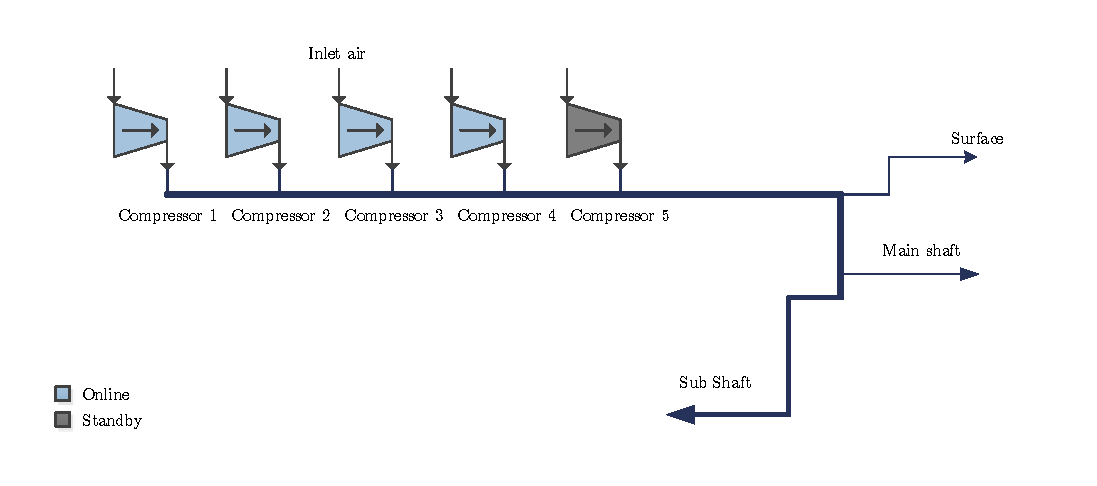
\includegraphics[trim =0.5cm 0.8cm 2.5cm 0.2cm,width=\textwidth]{Graphs/4/KUSLayout1/KUSLayout1.pdf}}
		\caption{Process schematic of the compressed air network}
		\label{fig: KUS Air layout}
	\end{figure}
\clearpage

\subsection{Model development}
	
From the investigation, the compressed air network was modelled in \gls{ptb}. The methodology described in Chapter 3 was utilised in this process. The following assumptions made to simplify the model development:
\begin{itemize}
	\item After cooling reduced compressed air temperature from $ 60 ^o $ \gls{c} to $ 40 ^o $ \gls{c}
	\item Underground temperature and humidity remained constant for each level
\end{itemize}
 The boundaries of the baseline simulation were selected based on the available data for the network. The developed simulation model is shown in \Cref{fig: KUS Baseline model}. For maximum accuracy, the simulation step size was set to the two minutes to match the resolution available from the data source.
The model components were calibrated so that the simulated outputs matched data from the real system. The process flow diagram for the simulation is shown in \Cref{fig: KUS Baseline model}. The model data inputs and outputs are described in \Cref{table: Mine A inputs/outputs}.

\begin{table}[h!]
	\centering
	\begin{tabular}{ll}
		\hline 
		Inputs \hspace*{4cm} & Outputs \hspace*{4cm} \\ \hhline{==}
		Level measured flows & Compressor powers \\
		Compressor schedules & Network flows \\
		Set-points & Network pressures \\
		\hline
	\end{tabular}
		\caption{Simulation inputs and outputs}
\label{table: Mine B inputs/outputs}
\end{table}
	
	\subsubsection{Verification of baseline simulation}
	Using the verification methodology, the simulation model verified by comparing the simulation outputs to actual measured values. The compressors outlet pressure often does not match the set-point. The measured outlet pressure was used as set points for the compressors to verify the power and flow outputs. The setpoints ensured that the pressure in the network is identical to that of the actual system as shown in \Cref{fig: Verification Pressure kusasalethu}.
	\par 
	\begin{figure}[h!]
		\centering
		% GNUPLOT: LaTeX picture with Postscript
\begingroup
  \makeatletter
  \providecommand\color[2][]{%
    \GenericError{(gnuplot) \space\space\space\@spaces}{%
      Package color not loaded in conjunction with
      terminal option `colourtext'%
    }{See the gnuplot documentation for explanation.%
    }{Either use 'blacktext' in gnuplot or load the package
      color.sty in LaTeX.}%
    \renewcommand\color[2][]{}%
  }%
  \providecommand\includegraphics[2][]{%
    \GenericError{(gnuplot) \space\space\space\@spaces}{%
      Package graphicx or graphics not loaded%
    }{See the gnuplot documentation for explanation.%
    }{The gnuplot epslatex terminal needs graphicx.sty or graphics.sty.}%
    \renewcommand\includegraphics[2][]{}%
  }%
  \providecommand\rotatebox[2]{#2}%
  \@ifundefined{ifGPcolor}{%
    \newif\ifGPcolor
    \GPcolortrue
  }{}%
  \@ifundefined{ifGPblacktext}{%
    \newif\ifGPblacktext
    \GPblacktextfalse
  }{}%
  % define a \g@addto@macro without @ in the name:
  \let\gplgaddtomacro\g@addto@macro
  % define empty templates for all commands taking text:
  \gdef\gplbacktext{}%
  \gdef\gplfronttext{}%
  \makeatother
  \ifGPblacktext
    % no textcolor at all
    \def\colorrgb#1{}%
    \def\colorgray#1{}%
  \else
    % gray or color?
    \ifGPcolor
      \def\colorrgb#1{\color[rgb]{#1}}%
      \def\colorgray#1{\color[gray]{#1}}%
      \expandafter\def\csname LTw\endcsname{\color{white}}%
      \expandafter\def\csname LTb\endcsname{\color{black}}%
      \expandafter\def\csname LTa\endcsname{\color{black}}%
      \expandafter\def\csname LT0\endcsname{\color[rgb]{1,0,0}}%
      \expandafter\def\csname LT1\endcsname{\color[rgb]{0,1,0}}%
      \expandafter\def\csname LT2\endcsname{\color[rgb]{0,0,1}}%
      \expandafter\def\csname LT3\endcsname{\color[rgb]{1,0,1}}%
      \expandafter\def\csname LT4\endcsname{\color[rgb]{0,1,1}}%
      \expandafter\def\csname LT5\endcsname{\color[rgb]{1,1,0}}%
      \expandafter\def\csname LT6\endcsname{\color[rgb]{0,0,0}}%
      \expandafter\def\csname LT7\endcsname{\color[rgb]{1,0.3,0}}%
      \expandafter\def\csname LT8\endcsname{\color[rgb]{0.5,0.5,0.5}}%
    \else
      % gray
      \def\colorrgb#1{\color{black}}%
      \def\colorgray#1{\color[gray]{#1}}%
      \expandafter\def\csname LTw\endcsname{\color{white}}%
      \expandafter\def\csname LTb\endcsname{\color{black}}%
      \expandafter\def\csname LTa\endcsname{\color{black}}%
      \expandafter\def\csname LT0\endcsname{\color{black}}%
      \expandafter\def\csname LT1\endcsname{\color{black}}%
      \expandafter\def\csname LT2\endcsname{\color{black}}%
      \expandafter\def\csname LT3\endcsname{\color{black}}%
      \expandafter\def\csname LT4\endcsname{\color{black}}%
      \expandafter\def\csname LT5\endcsname{\color{black}}%
      \expandafter\def\csname LT6\endcsname{\color{black}}%
      \expandafter\def\csname LT7\endcsname{\color{black}}%
      \expandafter\def\csname LT8\endcsname{\color{black}}%
    \fi
  \fi
    \setlength{\unitlength}{0.0500bp}%
    \ifx\gptboxheight\undefined%
      \newlength{\gptboxheight}%
      \newlength{\gptboxwidth}%
      \newsavebox{\gptboxtext}%
    \fi%
    \setlength{\fboxrule}{0.5pt}%
    \setlength{\fboxsep}{1pt}%
\begin{picture}(9360.00,2772.00)%
    \gplgaddtomacro\gplbacktext{%
      \colorrgb{0.00,0.00,0.00}%
      \put(814,924){\makebox(0,0)[r]{\strut{}$300$}}%
      \colorrgb{0.00,0.00,0.00}%
      \put(814,1452){\makebox(0,0)[r]{\strut{}$350$}}%
      \colorrgb{0.00,0.00,0.00}%
      \put(814,1979){\makebox(0,0)[r]{\strut{}$400$}}%
      \colorrgb{0.00,0.00,0.00}%
      \put(814,2507){\makebox(0,0)[r]{\strut{}$450$}}%
      \colorrgb{0.00,0.00,0.00}%
      \put(946,704){\makebox(0,0){\strut{}00:00}}%
      \colorrgb{0.00,0.00,0.00}%
      \put(2157,704){\makebox(0,0){\strut{}04:00}}%
      \colorrgb{0.00,0.00,0.00}%
      \put(3369,704){\makebox(0,0){\strut{}08:00}}%
      \colorrgb{0.00,0.00,0.00}%
      \put(4580,704){\makebox(0,0){\strut{}12:00}}%
      \colorrgb{0.00,0.00,0.00}%
      \put(5791,704){\makebox(0,0){\strut{}16:00}}%
      \colorrgb{0.00,0.00,0.00}%
      \put(7003,704){\makebox(0,0){\strut{}20:00}}%
      \colorrgb{0.00,0.00,0.00}%
      \put(8214,704){\makebox(0,0){\strut{}00:00}}%
      \colorrgb{0.00,0.00,0.00}%
      \put(8346,924){\makebox(0,0)[l]{\strut{}$0$}}%
      \colorrgb{0.00,0.00,0.00}%
      \put(8346,1557){\makebox(0,0)[l]{\strut{}$10$}}%
      \colorrgb{0.00,0.00,0.00}%
      \put(8346,2190){\makebox(0,0)[l]{\strut{}$20$}}%
    }%
    \gplgaddtomacro\gplfronttext{%
      \csname LTb\endcsname%
      \put(176,1715){\rotatebox{-270}{\makebox(0,0){\strut{}Pressure $(kPa)$}}}%
      \put(8851,1715){\rotatebox{-270}{\makebox(0,0){\strut{}$\% error$}}}%
      \put(4580,374){\makebox(0,0){\strut{}Time of Day}}%
      \csname LTb\endcsname%
      \put(2241,173){\makebox(0,0)[r]{\strut{}Baseline press.}}%
      \csname LTb\endcsname%
      \put(5208,173){\makebox(0,0)[r]{\strut{}Simulated press.}}%
      \csname LTb\endcsname%
      \put(8175,173){\makebox(0,0)[r]{\strut{}Error}}%
    }%
    \gplbacktext
    \put(0,0){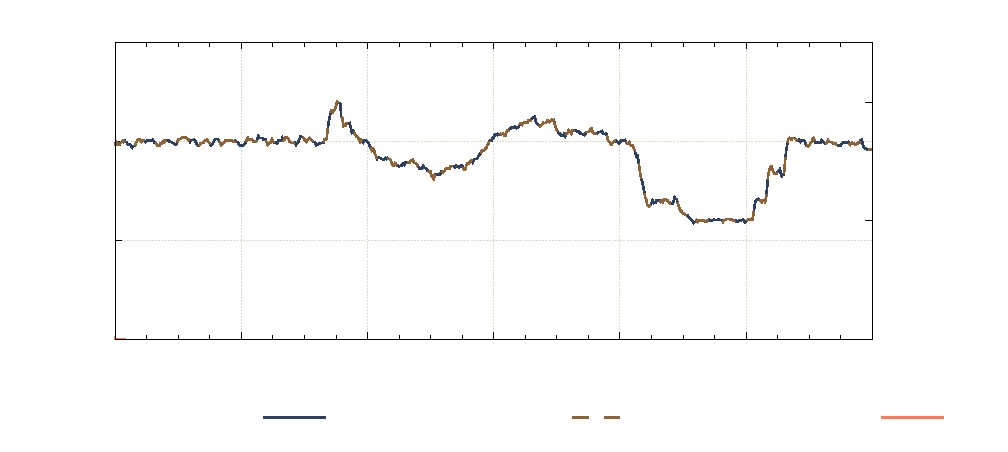
\includegraphics{Graphs/4/KusVerify/Pressure/Pressure}}%
    \gplfronttext
  \end{picture}%
\endgroup

		\caption{The compressor outlet pressure in the simulation compared to the actual measured pressure using actual measurements as setpoints}
		\label{fig: Verification Pressure kusasalethu}
	\end{figure}

 With the simulated pressure identical to the actual, the power and air-flow outputs were compared with outputs from the physical system. \Cref{fig: Verification Power kusasalethu} shows the comparison of the total power and flow of the system with the physically measured values for that same period. The accuracy of these parameters compared to the real system was $98.7 \%$ and $99.0 \%$ respectively. This simulation error was within the acceptable error limits.
 
 \begin{table}[h!]
 	\label{Kus verification table}
 	\centering
 	\begin{tabular}{p{0.5cm}p{8cm}p{5cm}r}
 		\hline
 		&Verification method & Result & $Err_{\%}$\\
 		\hhline{====}
 		\\ \multicolumn{4}{l}{\textbf{ Total Flow}}\\
 		&Residual Difference  & 0.22 kg/s & 0.53\% \\
 		&\gls{mae} 					 & 0.43 kg/s error & 1.02\% \\
 		&Coefficient of determination & $r^2 =0.99$ & -\\ 
 		\\ \multicolumn{4}{l}{\textbf{ Total power}}\\
 		&Residual Difference  & 0.05 MW & 0.39\% \\
 		&\gls{mae} 					 & 0.16 MW error & 1.36\% \\
 		&Coefficient of determination & $r^2 =0.91$ & -\\ 
 		\\ \multicolumn{4}{l}{\textbf{ Compressor outlet pressure}}\\
 		&Residual Difference  & 2.79 kPa & 0.71\% \\
 		&\gls{mae} 					 & 3.85 kPa error & 0.98\% \\
 		&Coefficient of determination & $r^2 =0.890$ & -\\
 		\\ 	\hline
 	\end{tabular} 
 	\caption{Verification of simulation model}
 \end{table}

	\begin{figure}[h!]
		\centering
		% GNUPLOT: LaTeX picture with Postscript
\begingroup
  \makeatletter
  \providecommand\color[2][]{%
    \GenericError{(gnuplot) \space\space\space\@spaces}{%
      Package color not loaded in conjunction with
      terminal option `colourtext'%
    }{See the gnuplot documentation for explanation.%
    }{Either use 'blacktext' in gnuplot or load the package
      color.sty in LaTeX.}%
    \renewcommand\color[2][]{}%
  }%
  \providecommand\includegraphics[2][]{%
    \GenericError{(gnuplot) \space\space\space\@spaces}{%
      Package graphicx or graphics not loaded%
    }{See the gnuplot documentation for explanation.%
    }{The gnuplot epslatex terminal needs graphicx.sty or graphics.sty.}%
    \renewcommand\includegraphics[2][]{}%
  }%
  \providecommand\rotatebox[2]{#2}%
  \@ifundefined{ifGPcolor}{%
    \newif\ifGPcolor
    \GPcolortrue
  }{}%
  \@ifundefined{ifGPblacktext}{%
    \newif\ifGPblacktext
    \GPblacktextfalse
  }{}%
  % define a \g@addto@macro without @ in the name:
  \let\gplgaddtomacro\g@addto@macro
  % define empty templates for all commands taking text:
  \gdef\gplbacktext{}%
  \gdef\gplfronttext{}%
  \makeatother
  \ifGPblacktext
    % no textcolor at all
    \def\colorrgb#1{}%
    \def\colorgray#1{}%
  \else
    % gray or color?
    \ifGPcolor
      \def\colorrgb#1{\color[rgb]{#1}}%
      \def\colorgray#1{\color[gray]{#1}}%
      \expandafter\def\csname LTw\endcsname{\color{white}}%
      \expandafter\def\csname LTb\endcsname{\color{black}}%
      \expandafter\def\csname LTa\endcsname{\color{black}}%
      \expandafter\def\csname LT0\endcsname{\color[rgb]{1,0,0}}%
      \expandafter\def\csname LT1\endcsname{\color[rgb]{0,1,0}}%
      \expandafter\def\csname LT2\endcsname{\color[rgb]{0,0,1}}%
      \expandafter\def\csname LT3\endcsname{\color[rgb]{1,0,1}}%
      \expandafter\def\csname LT4\endcsname{\color[rgb]{0,1,1}}%
      \expandafter\def\csname LT5\endcsname{\color[rgb]{1,1,0}}%
      \expandafter\def\csname LT6\endcsname{\color[rgb]{0,0,0}}%
      \expandafter\def\csname LT7\endcsname{\color[rgb]{1,0.3,0}}%
      \expandafter\def\csname LT8\endcsname{\color[rgb]{0.5,0.5,0.5}}%
    \else
      % gray
      \def\colorrgb#1{\color{black}}%
      \def\colorgray#1{\color[gray]{#1}}%
      \expandafter\def\csname LTw\endcsname{\color{white}}%
      \expandafter\def\csname LTb\endcsname{\color{black}}%
      \expandafter\def\csname LTa\endcsname{\color{black}}%
      \expandafter\def\csname LT0\endcsname{\color{black}}%
      \expandafter\def\csname LT1\endcsname{\color{black}}%
      \expandafter\def\csname LT2\endcsname{\color{black}}%
      \expandafter\def\csname LT3\endcsname{\color{black}}%
      \expandafter\def\csname LT4\endcsname{\color{black}}%
      \expandafter\def\csname LT5\endcsname{\color{black}}%
      \expandafter\def\csname LT6\endcsname{\color{black}}%
      \expandafter\def\csname LT7\endcsname{\color{black}}%
      \expandafter\def\csname LT8\endcsname{\color{black}}%
    \fi
  \fi
    \setlength{\unitlength}{0.0500bp}%
    \ifx\gptboxheight\undefined%
      \newlength{\gptboxheight}%
      \newlength{\gptboxwidth}%
      \newsavebox{\gptboxtext}%
    \fi%
    \setlength{\fboxrule}{0.5pt}%
    \setlength{\fboxsep}{1pt}%
\begin{picture}(9360.00,3276.00)%
    \gplgaddtomacro\gplbacktext{%
      \colorrgb{0.00,0.00,0.00}%
      \put(682,924){\makebox(0,0)[r]{\strut{}$30$}}%
      \colorrgb{0.00,0.00,0.00}%
      \put(682,1967){\makebox(0,0)[r]{\strut{}$40$}}%
      \colorrgb{0.00,0.00,0.00}%
      \put(682,3011){\makebox(0,0)[r]{\strut{}$50$}}%
      \colorrgb{0.00,0.00,0.00}%
      \put(814,704){\makebox(0,0){\strut{}00:00}}%
      \colorrgb{0.00,0.00,0.00}%
      \put(2047,704){\makebox(0,0){\strut{}04:00}}%
      \colorrgb{0.00,0.00,0.00}%
      \put(3281,704){\makebox(0,0){\strut{}08:00}}%
      \colorrgb{0.00,0.00,0.00}%
      \put(4514,704){\makebox(0,0){\strut{}12:00}}%
      \colorrgb{0.00,0.00,0.00}%
      \put(5747,704){\makebox(0,0){\strut{}16:00}}%
      \colorrgb{0.00,0.00,0.00}%
      \put(6981,704){\makebox(0,0){\strut{}20:00}}%
      \colorrgb{0.00,0.00,0.00}%
      \put(8214,704){\makebox(0,0){\strut{}00:00}}%
      \colorrgb{0.00,0.00,0.00}%
      \put(8346,924){\makebox(0,0)[l]{\strut{}$0$}}%
      \colorrgb{0.00,0.00,0.00}%
      \put(8346,1759){\makebox(0,0)[l]{\strut{}$10$}}%
      \colorrgb{0.00,0.00,0.00}%
      \put(8346,2594){\makebox(0,0)[l]{\strut{}$20$}}%
    }%
    \gplgaddtomacro\gplfronttext{%
      \csname LTb\endcsname%
      \put(176,1967){\rotatebox{-270}{\makebox(0,0){\strut{}flow $(kg/s)$}}}%
      \put(8851,1967){\rotatebox{-270}{\makebox(0,0){\strut{}$\% error$}}}%
      \put(4514,374){\makebox(0,0){\strut{}Time of Day}}%
      \csname LTb\endcsname%
      \put(2307,173){\makebox(0,0)[r]{\strut{}Baseline flow}}%
      \csname LTb\endcsname%
      \put(5010,173){\makebox(0,0)[r]{\strut{}Simulated flow}}%
      \csname LTb\endcsname%
      \put(7713,173){\makebox(0,0)[r]{\strut{}Error}}%
    }%
    \gplbacktext
    \put(0,0){\fbox{
\includegraphics[trim=0 0 0.1cm 0, clip]{Graphs/4/KusVerify/Flow/Flow}}}%
    \gplfronttext
  \end{picture}%
\endgroup

		(a)\\
		% GNUPLOT: LaTeX picture with Postscript
\begingroup
  \makeatletter
  \providecommand\color[2][]{%
    \GenericError{(gnuplot) \space\space\space\@spaces}{%
      Package color not loaded in conjunction with
      terminal option `colourtext'%
    }{See the gnuplot documentation for explanation.%
    }{Either use 'blacktext' in gnuplot or load the package
      color.sty in LaTeX.}%
    \renewcommand\color[2][]{}%
  }%
  \providecommand\includegraphics[2][]{%
    \GenericError{(gnuplot) \space\space\space\@spaces}{%
      Package graphicx or graphics not loaded%
    }{See the gnuplot documentation for explanation.%
    }{The gnuplot epslatex terminal needs graphicx.sty or graphics.sty.}%
    \renewcommand\includegraphics[2][]{}%
  }%
  \providecommand\rotatebox[2]{#2}%
  \@ifundefined{ifGPcolor}{%
    \newif\ifGPcolor
    \GPcolortrue
  }{}%
  \@ifundefined{ifGPblacktext}{%
    \newif\ifGPblacktext
    \GPblacktextfalse
  }{}%
  % define a \g@addto@macro without @ in the name:
  \let\gplgaddtomacro\g@addto@macro
  % define empty templates for all commands taking text:
  \gdef\gplbacktext{}%
  \gdef\gplfronttext{}%
  \makeatother
  \ifGPblacktext
    % no textcolor at all
    \def\colorrgb#1{}%
    \def\colorgray#1{}%
  \else
    % gray or color?
    \ifGPcolor
      \def\colorrgb#1{\color[rgb]{#1}}%
      \def\colorgray#1{\color[gray]{#1}}%
      \expandafter\def\csname LTw\endcsname{\color{white}}%
      \expandafter\def\csname LTb\endcsname{\color{black}}%
      \expandafter\def\csname LTa\endcsname{\color{black}}%
      \expandafter\def\csname LT0\endcsname{\color[rgb]{1,0,0}}%
      \expandafter\def\csname LT1\endcsname{\color[rgb]{0,1,0}}%
      \expandafter\def\csname LT2\endcsname{\color[rgb]{0,0,1}}%
      \expandafter\def\csname LT3\endcsname{\color[rgb]{1,0,1}}%
      \expandafter\def\csname LT4\endcsname{\color[rgb]{0,1,1}}%
      \expandafter\def\csname LT5\endcsname{\color[rgb]{1,1,0}}%
      \expandafter\def\csname LT6\endcsname{\color[rgb]{0,0,0}}%
      \expandafter\def\csname LT7\endcsname{\color[rgb]{1,0.3,0}}%
      \expandafter\def\csname LT8\endcsname{\color[rgb]{0.5,0.5,0.5}}%
    \else
      % gray
      \def\colorrgb#1{\color{black}}%
      \def\colorgray#1{\color[gray]{#1}}%
      \expandafter\def\csname LTw\endcsname{\color{white}}%
      \expandafter\def\csname LTb\endcsname{\color{black}}%
      \expandafter\def\csname LTa\endcsname{\color{black}}%
      \expandafter\def\csname LT0\endcsname{\color{black}}%
      \expandafter\def\csname LT1\endcsname{\color{black}}%
      \expandafter\def\csname LT2\endcsname{\color{black}}%
      \expandafter\def\csname LT3\endcsname{\color{black}}%
      \expandafter\def\csname LT4\endcsname{\color{black}}%
      \expandafter\def\csname LT5\endcsname{\color{black}}%
      \expandafter\def\csname LT6\endcsname{\color{black}}%
      \expandafter\def\csname LT7\endcsname{\color{black}}%
      \expandafter\def\csname LT8\endcsname{\color{black}}%
    \fi
  \fi
    \setlength{\unitlength}{0.0500bp}%
    \ifx\gptboxheight\undefined%
      \newlength{\gptboxheight}%
      \newlength{\gptboxwidth}%
      \newsavebox{\gptboxtext}%
    \fi%
    \setlength{\fboxrule}{0.5pt}%
    \setlength{\fboxsep}{1pt}%
\begin{picture}(9360.00,3276.00)%
    \gplgaddtomacro\gplbacktext{%
      \colorrgb{0.00,0.00,0.00}%
      \put(682,924){\makebox(0,0)[r]{\strut{}$8$}}%
      \colorrgb{0.00,0.00,0.00}%
      \put(682,1222){\makebox(0,0)[r]{\strut{}$9$}}%
      \colorrgb{0.00,0.00,0.00}%
      \put(682,1520){\makebox(0,0)[r]{\strut{}$10$}}%
      \colorrgb{0.00,0.00,0.00}%
      \put(682,1818){\makebox(0,0)[r]{\strut{}$11$}}%
      \colorrgb{0.00,0.00,0.00}%
      \put(682,2117){\makebox(0,0)[r]{\strut{}$12$}}%
      \colorrgb{0.00,0.00,0.00}%
      \put(682,2415){\makebox(0,0)[r]{\strut{}$13$}}%
      \colorrgb{0.00,0.00,0.00}%
      \put(682,2713){\makebox(0,0)[r]{\strut{}$14$}}%
      \colorrgb{0.00,0.00,0.00}%
      \put(682,3011){\makebox(0,0)[r]{\strut{}$15$}}%
      \colorrgb{0.00,0.00,0.00}%
      \put(814,704){\makebox(0,0){\strut{}00:00}}%
      \colorrgb{0.00,0.00,0.00}%
      \put(2047,704){\makebox(0,0){\strut{}04:00}}%
      \colorrgb{0.00,0.00,0.00}%
      \put(3281,704){\makebox(0,0){\strut{}08:00}}%
      \colorrgb{0.00,0.00,0.00}%
      \put(4514,704){\makebox(0,0){\strut{}12:00}}%
      \colorrgb{0.00,0.00,0.00}%
      \put(5747,704){\makebox(0,0){\strut{}16:00}}%
      \colorrgb{0.00,0.00,0.00}%
      \put(6981,704){\makebox(0,0){\strut{}20:00}}%
      \colorrgb{0.00,0.00,0.00}%
      \put(8214,704){\makebox(0,0){\strut{}00:00}}%
      \colorrgb{0.00,0.00,0.00}%
      \put(8346,924){\makebox(0,0)[l]{\strut{}$0$}}%
      \colorrgb{0.00,0.00,0.00}%
      \put(8346,1759){\makebox(0,0)[l]{\strut{}$10$}}%
      \colorrgb{0.00,0.00,0.00}%
      \put(8346,2594){\makebox(0,0)[l]{\strut{}$20$}}%
    }%
    \gplgaddtomacro\gplfronttext{%
      \csname LTb\endcsname%
      \put(176,1967){\rotatebox{-270}{\makebox(0,0){\strut{}Power $(MW)$}}}%
      \put(8851,1967){\rotatebox{-270}{\makebox(0,0){\strut{}$\% error$}}}%
      \put(4514,374){\makebox(0,0){\strut{}Time of Day}}%
      \csname LTb\endcsname%
      \put(2241,173){\makebox(0,0)[r]{\strut{}Baseline power}}%
      \csname LTb\endcsname%
      \put(5076,173){\makebox(0,0)[r]{\strut{}Simulated power}}%
      \csname LTb\endcsname%
      \put(7911,173){\makebox(0,0)[r]{\strut{}Error}}%
    }%
    \gplbacktext
    \put(0,0){\fbox{
\includegraphics[trim=0 0 0.1cm 0, clip]{Graphs/4/KusVerify/Power/Power}}}%
    \gplfronttext
  \end{picture}%
\endgroup

		(b)\\
		\caption{Verification of the total (a) flow and (b) power of the system}
		\label{fig: Verification Power kusasalethu}
	\end{figure}

	Once the power and flow parameters were verified with an acceptable error, the actual pressure set-point profile was imported to the compressor controllers. The simulated outlet pressure was then compared to the actual measured pressure and setpoint; this is shown in \Cref{fig: Verification Pressure kusasalethu Setpoint}. The accuracy of the compressor outlet pressure was acceptable at 99.02 \%. The measured flows for all measured subcomponents were independently verified to ensure system accuracy. A comparison between simulation outputs and physical measurements is shown in \Cref{Table: B verification}.

	\begin{figure}[h!]
		\centering
		% GNUPLOT: LaTeX picture with Postscript
\begingroup
  \makeatletter
  \providecommand\color[2][]{%
    \GenericError{(gnuplot) \space\space\space\@spaces}{%
      Package color not loaded in conjunction with
      terminal option `colourtext'%
    }{See the gnuplot documentation for explanation.%
    }{Either use 'blacktext' in gnuplot or load the package
      color.sty in LaTeX.}%
    \renewcommand\color[2][]{}%
  }%
  \providecommand\includegraphics[2][]{%
    \GenericError{(gnuplot) \space\space\space\@spaces}{%
      Package graphicx or graphics not loaded%
    }{See the gnuplot documentation for explanation.%
    }{The gnuplot epslatex terminal needs graphicx.sty or graphics.sty.}%
    \renewcommand\includegraphics[2][]{}%
  }%
  \providecommand\rotatebox[2]{#2}%
  \@ifundefined{ifGPcolor}{%
    \newif\ifGPcolor
    \GPcolortrue
  }{}%
  \@ifundefined{ifGPblacktext}{%
    \newif\ifGPblacktext
    \GPblacktextfalse
  }{}%
  % define a \g@addto@macro without @ in the name:
  \let\gplgaddtomacro\g@addto@macro
  % define empty templates for all commands taking text:
  \gdef\gplbacktext{}%
  \gdef\gplfronttext{}%
  \makeatother
  \ifGPblacktext
    % no textcolor at all
    \def\colorrgb#1{}%
    \def\colorgray#1{}%
  \else
    % gray or color?
    \ifGPcolor
      \def\colorrgb#1{\color[rgb]{#1}}%
      \def\colorgray#1{\color[gray]{#1}}%
      \expandafter\def\csname LTw\endcsname{\color{white}}%
      \expandafter\def\csname LTb\endcsname{\color{black}}%
      \expandafter\def\csname LTa\endcsname{\color{black}}%
      \expandafter\def\csname LT0\endcsname{\color[rgb]{1,0,0}}%
      \expandafter\def\csname LT1\endcsname{\color[rgb]{0,1,0}}%
      \expandafter\def\csname LT2\endcsname{\color[rgb]{0,0,1}}%
      \expandafter\def\csname LT3\endcsname{\color[rgb]{1,0,1}}%
      \expandafter\def\csname LT4\endcsname{\color[rgb]{0,1,1}}%
      \expandafter\def\csname LT5\endcsname{\color[rgb]{1,1,0}}%
      \expandafter\def\csname LT6\endcsname{\color[rgb]{0,0,0}}%
      \expandafter\def\csname LT7\endcsname{\color[rgb]{1,0.3,0}}%
      \expandafter\def\csname LT8\endcsname{\color[rgb]{0.5,0.5,0.5}}%
    \else
      % gray
      \def\colorrgb#1{\color{black}}%
      \def\colorgray#1{\color[gray]{#1}}%
      \expandafter\def\csname LTw\endcsname{\color{white}}%
      \expandafter\def\csname LTb\endcsname{\color{black}}%
      \expandafter\def\csname LTa\endcsname{\color{black}}%
      \expandafter\def\csname LT0\endcsname{\color{black}}%
      \expandafter\def\csname LT1\endcsname{\color{black}}%
      \expandafter\def\csname LT2\endcsname{\color{black}}%
      \expandafter\def\csname LT3\endcsname{\color{black}}%
      \expandafter\def\csname LT4\endcsname{\color{black}}%
      \expandafter\def\csname LT5\endcsname{\color{black}}%
      \expandafter\def\csname LT6\endcsname{\color{black}}%
      \expandafter\def\csname LT7\endcsname{\color{black}}%
      \expandafter\def\csname LT8\endcsname{\color{black}}%
    \fi
  \fi
    \setlength{\unitlength}{0.0500bp}%
    \ifx\gptboxheight\undefined%
      \newlength{\gptboxheight}%
      \newlength{\gptboxwidth}%
      \newsavebox{\gptboxtext}%
    \fi%
    \setlength{\fboxrule}{0.5pt}%
    \setlength{\fboxsep}{1pt}%
\begin{picture}(9360.00,4032.00)%
    \gplgaddtomacro\gplbacktext{%
      \colorrgb{0.00,0.00,0.00}%
      \put(814,1144){\makebox(0,0)[r]{\strut{}$300$}}%
      \colorrgb{0.00,0.00,0.00}%
      \put(814,2018){\makebox(0,0)[r]{\strut{}$350$}}%
      \colorrgb{0.00,0.00,0.00}%
      \put(814,2893){\makebox(0,0)[r]{\strut{}$400$}}%
      \colorrgb{0.00,0.00,0.00}%
      \put(814,3767){\makebox(0,0)[r]{\strut{}$450$}}%
      \colorrgb{0.00,0.00,0.00}%
      \put(946,924){\makebox(0,0){\strut{}00:00}}%
      \colorrgb{0.00,0.00,0.00}%
      \put(2157,924){\makebox(0,0){\strut{}04:00}}%
      \colorrgb{0.00,0.00,0.00}%
      \put(3369,924){\makebox(0,0){\strut{}08:00}}%
      \colorrgb{0.00,0.00,0.00}%
      \put(4580,924){\makebox(0,0){\strut{}12:00}}%
      \colorrgb{0.00,0.00,0.00}%
      \put(5791,924){\makebox(0,0){\strut{}16:00}}%
      \colorrgb{0.00,0.00,0.00}%
      \put(7003,924){\makebox(0,0){\strut{}20:00}}%
      \colorrgb{0.00,0.00,0.00}%
      \put(8214,924){\makebox(0,0){\strut{}00:00}}%
      \colorrgb{0.00,0.00,0.00}%
      \put(8346,1144){\makebox(0,0)[l]{\strut{}$0$}}%
      \colorrgb{0.00,0.00,0.00}%
      \put(8346,2193){\makebox(0,0)[l]{\strut{}$10$}}%
      \colorrgb{0.00,0.00,0.00}%
      \put(8346,3242){\makebox(0,0)[l]{\strut{}$20$}}%
    }%
    \gplgaddtomacro\gplfronttext{%
      \csname LTb\endcsname%
      \put(176,2455){\rotatebox{-270}{\makebox(0,0){\strut{}Pressure $(kPa)$}}}%
      \put(8851,2455){\rotatebox{-270}{\makebox(0,0){\strut{}$\% error$}}}%
      \put(4580,594){\makebox(0,0){\strut{}Time of Day}}%
      \csname LTb\endcsname%
      \put(3725,393){\makebox(0,0)[r]{\strut{}Actual}}%
      \csname LTb\endcsname%
      \put(3725,173){\makebox(0,0)[r]{\strut{}Simulation.}}%
      \csname LTb\endcsname%
      \put(6032,393){\makebox(0,0)[r]{\strut{}Set-point}}%
      \csname LTb\endcsname%
      \put(5900,173){\makebox(0,0)[r]{\strut{}Rel. Error}}%
    }%
    \gplbacktext
    \put(0,0){\fbox{
\includegraphics[trim=0 0 0.1cm 0, clip]{Graphs/4/KusVerify/Pressure2/Pressure2}}}%
    \gplfronttext
  \end{picture}%
\endgroup

		\caption{Verifying the pressure response of the system given the pressure set points as inputs}
		\label{fig: Verification Pressure kusasalethu Setpoint}
	\end{figure}
	\subsection{Scenario 1. Refuge bay optimisation}
	After an underground investigation, unnecessary refuge bay leaks were identified as a significant inefficiency that can be reduced. A test on a single mining level was performed to measure the potential flow saving of reducing refuge bay leaks. The test showed that by reducing refuge bay leaks, by closing the valves, would lead to an average air saving of $0.05$ $kg/s$ per refuge bay at normal operational pressures. This measurement was conservative as it was not possible to close all the refuge bays on the level for the test. 
	\par 
	Due to the size of the mine, extending these tests to include the rest of the mining sections was not practical.  Therefore,  the benefits of an intervention on the entire mine could not accurately be determined from practical tests. Using simulation the typical operation with can be accurately compared with the intervention scenario to quantify the potential financial and operational benefits throughout a given period.
	\par
	The simulation model boundaries were updated to include refuge bay leaks on each level. For each refuge chamber, an air leak was added to the model by utilising per level layouts indicating locations of refuge bays. These leaks were modelled as flow demands using the data from the initial refuge bay tests. The overall mass flow of the system was maintained to ensure model accuracy. T By adding the flow component in the actual location in the process, the pressure is each chamber is correctly modelled. The full simulation model is shown in \Cref{fig: Refuge bay layout}. The updated simulation model was re-checked to ensure accuracy. This model was used as a baseline to quantify saving for the scenario.
	\par 
	Recreating the optimised scenario was modelled by setting the refuge bay flow components to 0 $kg/s$. The simulation was performed and the output data compared to the baseline. \Cref{fig: RefugeBay Power.} shows the baseline power compared to the optimised scenario. The comparison showed a potential 0.92 MW improvement in \gls{ee} through optimisation of refuge bay leaks. The optimised scenario would lead to R5.13M in energy cost saving for the mine.
	\par
	\begin{figure}[h!]
		\centering
		% GNUPLOT: LaTeX picture with Postscript
\begingroup
  \makeatletter
  \providecommand\color[2][]{%
    \GenericError{(gnuplot) \space\space\space\@spaces}{%
      Package color not loaded in conjunction with
      terminal option `colourtext'%
    }{See the gnuplot documentation for explanation.%
    }{Either use 'blacktext' in gnuplot or load the package
      color.sty in LaTeX.}%
    \renewcommand\color[2][]{}%
  }%
  \providecommand\includegraphics[2][]{%
    \GenericError{(gnuplot) \space\space\space\@spaces}{%
      Package graphicx or graphics not loaded%
    }{See the gnuplot documentation for explanation.%
    }{The gnuplot epslatex terminal needs graphicx.sty or graphics.sty.}%
    \renewcommand\includegraphics[2][]{}%
  }%
  \providecommand\rotatebox[2]{#2}%
  \@ifundefined{ifGPcolor}{%
    \newif\ifGPcolor
    \GPcolortrue
  }{}%
  \@ifundefined{ifGPblacktext}{%
    \newif\ifGPblacktext
    \GPblacktextfalse
  }{}%
  % define a \g@addto@macro without @ in the name:
  \let\gplgaddtomacro\g@addto@macro
  % define empty templates for all commands taking text:
  \gdef\gplbacktext{}%
  \gdef\gplfronttext{}%
  \makeatother
  \ifGPblacktext
    % no textcolor at all
    \def\colorrgb#1{}%
    \def\colorgray#1{}%
  \else
    % gray or color?
    \ifGPcolor
      \def\colorrgb#1{\color[rgb]{#1}}%
      \def\colorgray#1{\color[gray]{#1}}%
      \expandafter\def\csname LTw\endcsname{\color{white}}%
      \expandafter\def\csname LTb\endcsname{\color{black}}%
      \expandafter\def\csname LTa\endcsname{\color{black}}%
      \expandafter\def\csname LT0\endcsname{\color[rgb]{1,0,0}}%
      \expandafter\def\csname LT1\endcsname{\color[rgb]{0,1,0}}%
      \expandafter\def\csname LT2\endcsname{\color[rgb]{0,0,1}}%
      \expandafter\def\csname LT3\endcsname{\color[rgb]{1,0,1}}%
      \expandafter\def\csname LT4\endcsname{\color[rgb]{0,1,1}}%
      \expandafter\def\csname LT5\endcsname{\color[rgb]{1,1,0}}%
      \expandafter\def\csname LT6\endcsname{\color[rgb]{0,0,0}}%
      \expandafter\def\csname LT7\endcsname{\color[rgb]{1,0.3,0}}%
      \expandafter\def\csname LT8\endcsname{\color[rgb]{0.5,0.5,0.5}}%
    \else
      % gray
      \def\colorrgb#1{\color{black}}%
      \def\colorgray#1{\color[gray]{#1}}%
      \expandafter\def\csname LTw\endcsname{\color{white}}%
      \expandafter\def\csname LTb\endcsname{\color{black}}%
      \expandafter\def\csname LTa\endcsname{\color{black}}%
      \expandafter\def\csname LT0\endcsname{\color{black}}%
      \expandafter\def\csname LT1\endcsname{\color{black}}%
      \expandafter\def\csname LT2\endcsname{\color{black}}%
      \expandafter\def\csname LT3\endcsname{\color{black}}%
      \expandafter\def\csname LT4\endcsname{\color{black}}%
      \expandafter\def\csname LT5\endcsname{\color{black}}%
      \expandafter\def\csname LT6\endcsname{\color{black}}%
      \expandafter\def\csname LT7\endcsname{\color{black}}%
      \expandafter\def\csname LT8\endcsname{\color{black}}%
    \fi
  \fi
    \setlength{\unitlength}{0.0500bp}%
    \ifx\gptboxheight\undefined%
      \newlength{\gptboxheight}%
      \newlength{\gptboxwidth}%
      \newsavebox{\gptboxtext}%
    \fi%
    \setlength{\fboxrule}{0.5pt}%
    \setlength{\fboxsep}{1pt}%
\begin{picture}(9360.00,3780.00)%
    \gplgaddtomacro\gplbacktext{%
      \colorrgb{0.00,0.00,0.00}%
      \put(682,924){\makebox(0,0)[r]{\strut{}$0$}}%
      \colorrgb{0.00,0.00,0.00}%
      \put(682,1788){\makebox(0,0)[r]{\strut{}$5$}}%
      \colorrgb{0.00,0.00,0.00}%
      \put(682,2651){\makebox(0,0)[r]{\strut{}$10$}}%
      \colorrgb{0.00,0.00,0.00}%
      \put(682,3515){\makebox(0,0)[r]{\strut{}$15$}}%
      \colorrgb{0.00,0.00,0.00}%
      \put(814,704){\makebox(0,0){\strut{}00:00}}%
      \colorrgb{0.00,0.00,0.00}%
      \put(2172,704){\makebox(0,0){\strut{}04:00}}%
      \colorrgb{0.00,0.00,0.00}%
      \put(3530,704){\makebox(0,0){\strut{}08:00}}%
      \colorrgb{0.00,0.00,0.00}%
      \put(4888,704){\makebox(0,0){\strut{}12:00}}%
      \colorrgb{0.00,0.00,0.00}%
      \put(6246,704){\makebox(0,0){\strut{}16:00}}%
      \colorrgb{0.00,0.00,0.00}%
      \put(7604,704){\makebox(0,0){\strut{}20:00}}%
      \colorrgb{0.00,0.00,0.00}%
      \put(8962,704){\makebox(0,0){\strut{}00:00}}%
    }%
    \gplgaddtomacro\gplfronttext{%
      \csname LTb\endcsname%
      \put(176,2219){\rotatebox{-270}{\makebox(0,0){\strut{}Power $(MW)$}}}%
      \put(4888,374){\makebox(0,0){\strut{}Time of Day}}%
      \csname LTb\endcsname%
      \put(2813,173){\makebox(0,0)[r]{\strut{}Baseline}}%
      \csname LTb\endcsname%
      \put(5252,173){\makebox(0,0)[r]{\strut{}Intervention}}%
      \csname LTb\endcsname%
      \put(7691,173){\makebox(0,0)[r]{\strut{}Power saving}}%
    }%
    \gplbacktext
    \put(0,0){
\includegraphics{Graphs/4/KUSResults/RefugePower/RefugePower}}%
    \gplfronttext
  \end{picture}%
\endgroup

		\caption{The baseline system power compared to the system power when refuge bay leaks are reduced}
		\label{fig: RefugeBay Power.}
	\end{figure} 
	An additional pressure benefit was identified during the drilling shift, shown in \Cref{fig: RefugeBay Pressures.}. The reduced flow leads to a pressure increase of about 15 \glssymbol{kpa}. The pressure increase could lead to an increase in drilling efficiency.
	\begin{figure}[h!]
		\centering
		% GNUPLOT: LaTeX picture with Postscript
\begingroup
  \makeatletter
  \providecommand\color[2][]{%
    \GenericError{(gnuplot) \space\space\space\@spaces}{%
      Package color not loaded in conjunction with
      terminal option `colourtext'%
    }{See the gnuplot documentation for explanation.%
    }{Either use 'blacktext' in gnuplot or load the package
      color.sty in LaTeX.}%
    \renewcommand\color[2][]{}%
  }%
  \providecommand\includegraphics[2][]{%
    \GenericError{(gnuplot) \space\space\space\@spaces}{%
      Package graphicx or graphics not loaded%
    }{See the gnuplot documentation for explanation.%
    }{The gnuplot epslatex terminal needs graphicx.sty or graphics.sty.}%
    \renewcommand\includegraphics[2][]{}%
  }%
  \providecommand\rotatebox[2]{#2}%
  \@ifundefined{ifGPcolor}{%
    \newif\ifGPcolor
    \GPcolortrue
  }{}%
  \@ifundefined{ifGPblacktext}{%
    \newif\ifGPblacktext
    \GPblacktextfalse
  }{}%
  % define a \g@addto@macro without @ in the name:
  \let\gplgaddtomacro\g@addto@macro
  % define empty templates for all commands taking text:
  \gdef\gplbacktext{}%
  \gdef\gplfronttext{}%
  \makeatother
  \ifGPblacktext
    % no textcolor at all
    \def\colorrgb#1{}%
    \def\colorgray#1{}%
  \else
    % gray or color?
    \ifGPcolor
      \def\colorrgb#1{\color[rgb]{#1}}%
      \def\colorgray#1{\color[gray]{#1}}%
      \expandafter\def\csname LTw\endcsname{\color{white}}%
      \expandafter\def\csname LTb\endcsname{\color{black}}%
      \expandafter\def\csname LTa\endcsname{\color{black}}%
      \expandafter\def\csname LT0\endcsname{\color[rgb]{1,0,0}}%
      \expandafter\def\csname LT1\endcsname{\color[rgb]{0,1,0}}%
      \expandafter\def\csname LT2\endcsname{\color[rgb]{0,0,1}}%
      \expandafter\def\csname LT3\endcsname{\color[rgb]{1,0,1}}%
      \expandafter\def\csname LT4\endcsname{\color[rgb]{0,1,1}}%
      \expandafter\def\csname LT5\endcsname{\color[rgb]{1,1,0}}%
      \expandafter\def\csname LT6\endcsname{\color[rgb]{0,0,0}}%
      \expandafter\def\csname LT7\endcsname{\color[rgb]{1,0.3,0}}%
      \expandafter\def\csname LT8\endcsname{\color[rgb]{0.5,0.5,0.5}}%
    \else
      % gray
      \def\colorrgb#1{\color{black}}%
      \def\colorgray#1{\color[gray]{#1}}%
      \expandafter\def\csname LTw\endcsname{\color{white}}%
      \expandafter\def\csname LTb\endcsname{\color{black}}%
      \expandafter\def\csname LTa\endcsname{\color{black}}%
      \expandafter\def\csname LT0\endcsname{\color{black}}%
      \expandafter\def\csname LT1\endcsname{\color{black}}%
      \expandafter\def\csname LT2\endcsname{\color{black}}%
      \expandafter\def\csname LT3\endcsname{\color{black}}%
      \expandafter\def\csname LT4\endcsname{\color{black}}%
      \expandafter\def\csname LT5\endcsname{\color{black}}%
      \expandafter\def\csname LT6\endcsname{\color{black}}%
      \expandafter\def\csname LT7\endcsname{\color{black}}%
      \expandafter\def\csname LT8\endcsname{\color{black}}%
    \fi
  \fi
    \setlength{\unitlength}{0.0500bp}%
    \ifx\gptboxheight\undefined%
      \newlength{\gptboxheight}%
      \newlength{\gptboxwidth}%
      \newsavebox{\gptboxtext}%
    \fi%
    \setlength{\fboxrule}{0.5pt}%
    \setlength{\fboxsep}{1pt}%
\begin{picture}(9360.00,3780.00)%
    \gplgaddtomacro\gplbacktext{%
      \colorrgb{0.00,0.00,0.00}%
      \put(814,1183){\makebox(0,0)[r]{\strut{}$360$}}%
      \colorrgb{0.00,0.00,0.00}%
      \put(814,1701){\makebox(0,0)[r]{\strut{}$380$}}%
      \colorrgb{0.00,0.00,0.00}%
      \put(814,2220){\makebox(0,0)[r]{\strut{}$400$}}%
      \colorrgb{0.00,0.00,0.00}%
      \put(814,2738){\makebox(0,0)[r]{\strut{}$420$}}%
      \colorrgb{0.00,0.00,0.00}%
      \put(814,3256){\makebox(0,0)[r]{\strut{}$440$}}%
      \colorrgb{0.00,0.00,0.00}%
      \put(946,704){\makebox(0,0){\strut{}00:00}}%
      \colorrgb{0.00,0.00,0.00}%
      \put(2282,704){\makebox(0,0){\strut{}04:00}}%
      \colorrgb{0.00,0.00,0.00}%
      \put(3618,704){\makebox(0,0){\strut{}08:00}}%
      \colorrgb{0.00,0.00,0.00}%
      \put(4954,704){\makebox(0,0){\strut{}12:00}}%
      \colorrgb{0.00,0.00,0.00}%
      \put(6290,704){\makebox(0,0){\strut{}16:00}}%
      \colorrgb{0.00,0.00,0.00}%
      \put(7626,704){\makebox(0,0){\strut{}20:00}}%
      \colorrgb{0.00,0.00,0.00}%
      \put(8962,704){\makebox(0,0){\strut{}00:00}}%
    }%
    \gplgaddtomacro\gplfronttext{%
      \csname LTb\endcsname%
      \put(176,2219){\rotatebox{-270}{\makebox(0,0){\strut{}Pressure $(kPa)$}}}%
      \put(4954,374){\makebox(0,0){\strut{}Time of Day}}%
      \csname LTb\endcsname%
      \put(4099,173){\makebox(0,0)[r]{\strut{}Baseline}}%
      \csname LTb\endcsname%
      \put(6538,173){\makebox(0,0)[r]{\strut{}Intervention}}%
    }%
    \gplbacktext
    \put(0,0){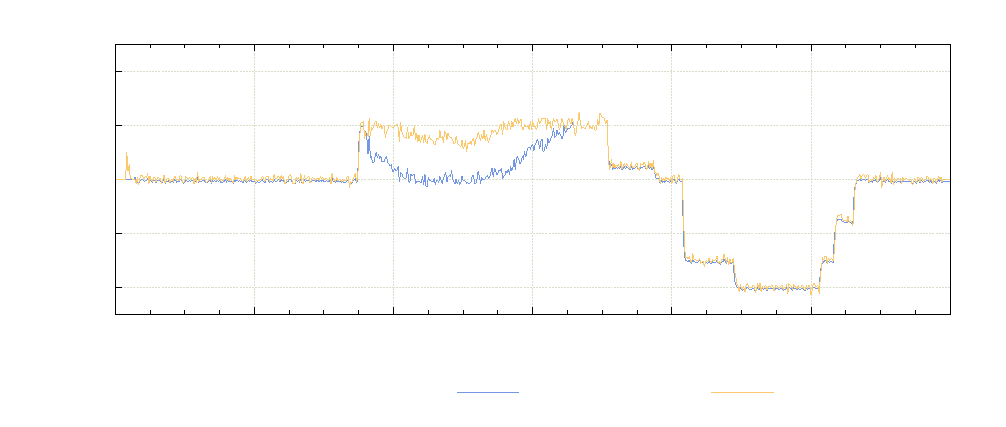
\includegraphics{Graphs/4/KUSResults/RefugePressure/RefugePressure}}%
    \gplfronttext
  \end{picture}%
\endgroup

		\caption{The baseline system pressure relative to the system pressure when refuge bay leaks are reduced}
		\label{fig: RefugeBay Pressures.}
	\end{figure} 
	\subsection{Scenario 2. Closing off levels and inactive work areas}
	\subsubsection{Scenario background}
	The largest impact on energy costs can be achieved during the energy high demand time periods. At mine B, blasting coincides with the evening energy demand peak. Typically, the air requirement during this period is lowered. However, due to compressed air misuse, leaks and open valves, significant amounts of air is still used during this time. Reducing pressure to areas during these times may lead to a major power and cost saving. 
	\par 
	Closing off stope valves and reducing station pressure were identified as two strategies to reduce airflow during the evening peak. The station cannot be closed completely as some services still require the air supply. 
	\par 
	Simulations were performed to identify the most suitable strategy and to quantify the effect of each on a single mining level. The level was modelled to include all the main leaks, refuge bays and drilling sections.  
	\subsubsection{Underground investigation}
	The components of the modelled were calibrated using manual measurements from an investigation of a mining level. A walkthrough inspection of the level was performed. Air users, leaks and inefficiencies were identified, quantified and mapped; the resultant schematic is provided in Appendix \ref{Manualinvestigation}.
	\par 
	A simulation schematic for the level was developed using the information from the level investigation. The simulation process schematic is shown in \Cref{fig: KUS Simulation level layout}. The results of the single level simulation can be expanded to other levels to obtain the total potential improvement that can be achieved.
	\begin{figure}[h!]
		\centering
		\fbox{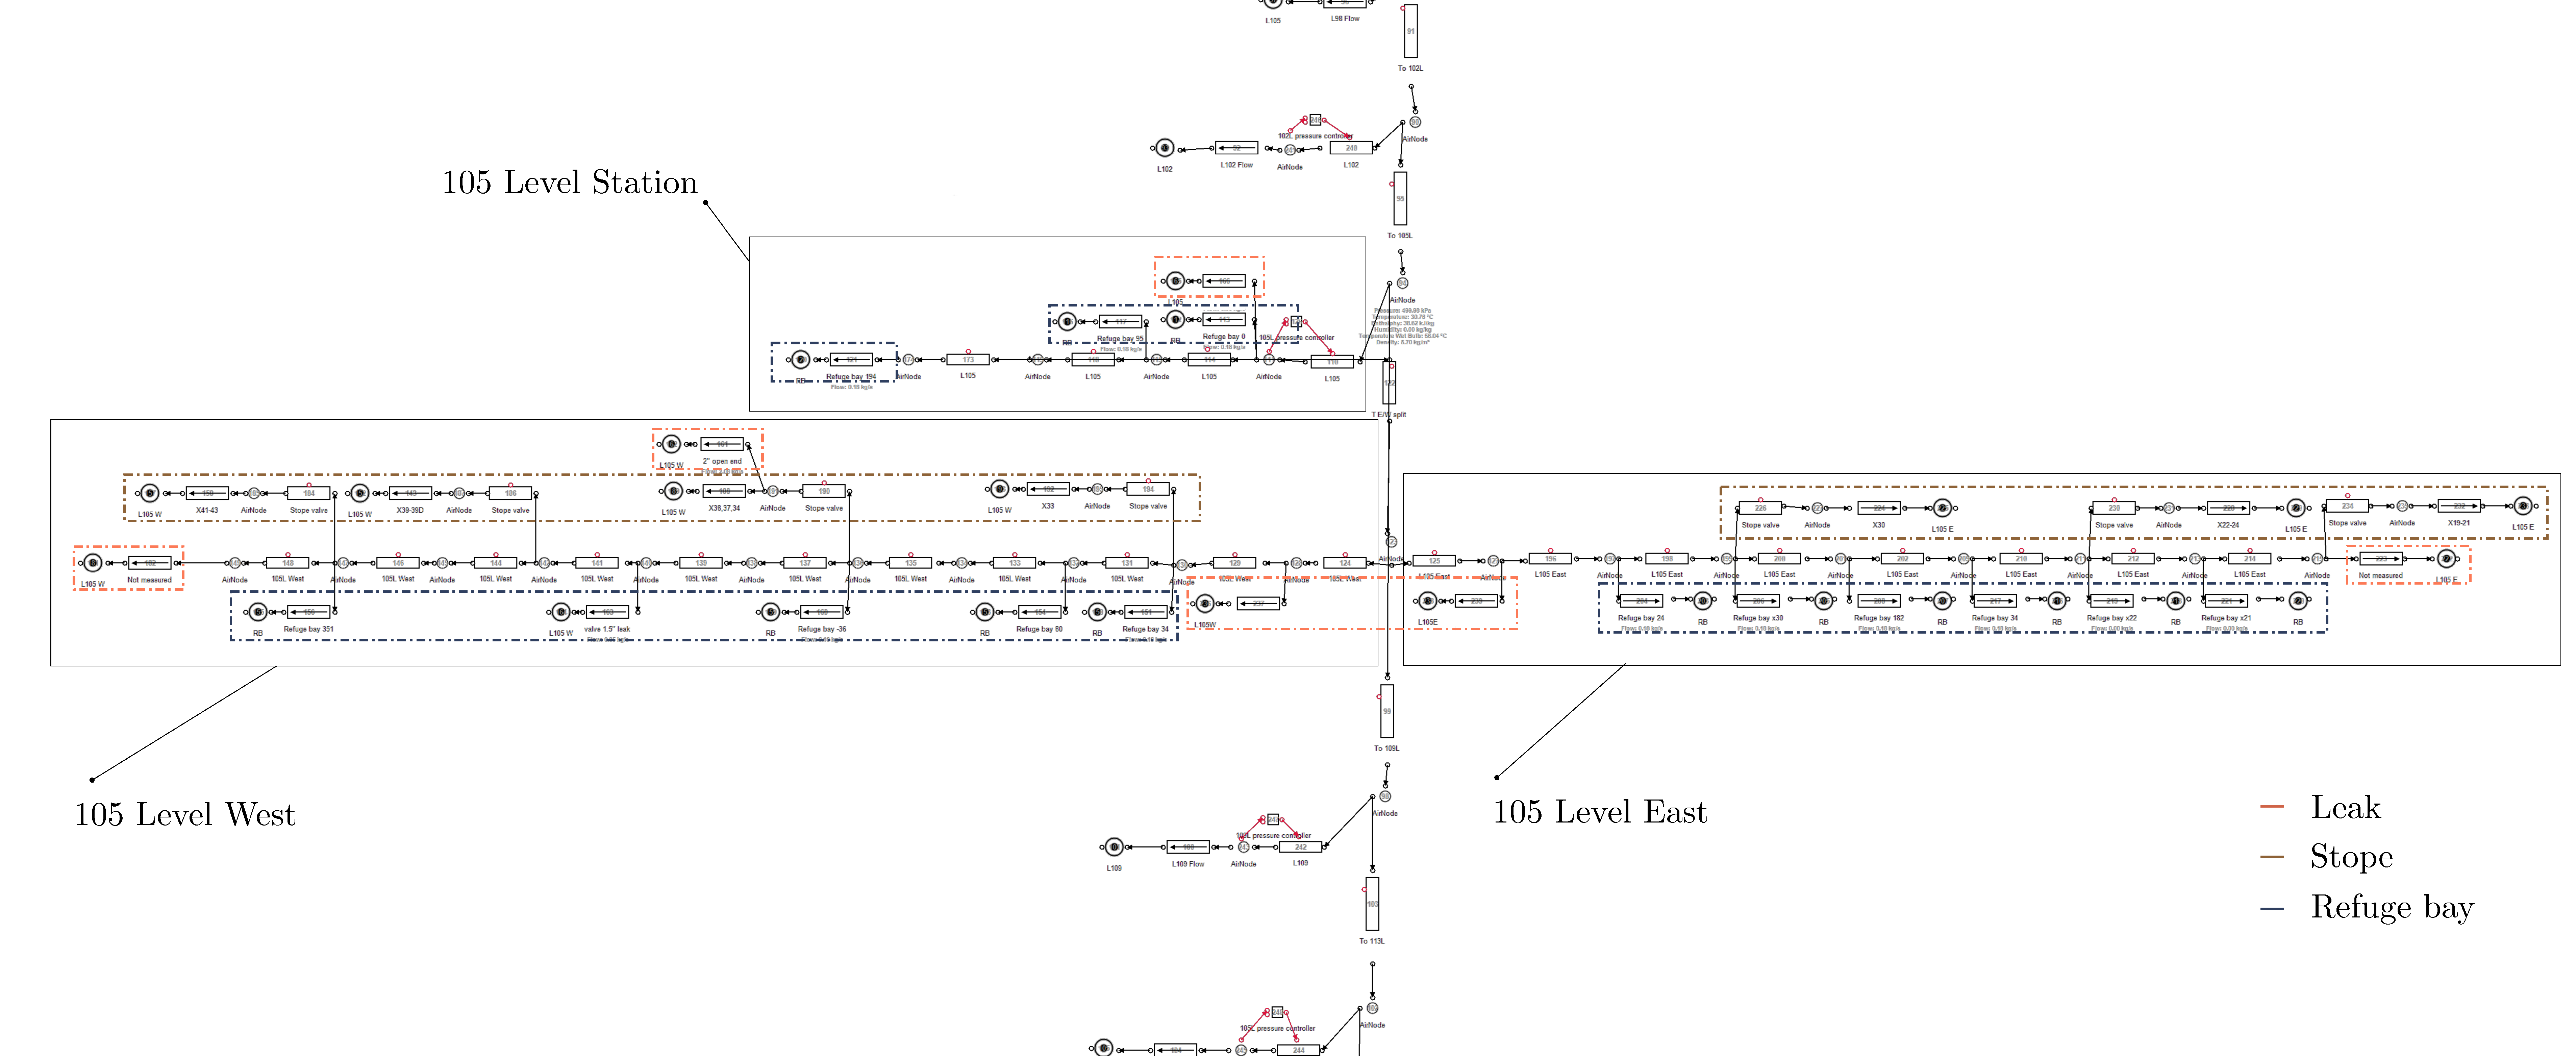
\includegraphics[angle=90,trim = 0 20cm 0 80cm, clip,height=0.95\textheight]{Images/A/StopeSim}}
		\caption{Underground level layout}
		\label{fig: KUS Simulation level layout}
	\end{figure}	
	\clearpage
	\subsubsection{Simulated results}
	Station control, in-stope control and a combination were simulated were all simulated for 105L. Station control means control of the pressure of at the station of the level. In-stope control is control of the is cut the airflow to the mining section during certain periods. \Cref{fig: 105 Flow savings} shows the effect the various interventions have on the flow for 105L compared to the baseline.

	\begin{figure}[h!]
		\centering
		% GNUPLOT: LaTeX picture with Postscript
\begingroup
  \makeatletter
  \providecommand\color[2][]{%
    \GenericError{(gnuplot) \space\space\space\@spaces}{%
      Package color not loaded in conjunction with
      terminal option `colourtext'%
    }{See the gnuplot documentation for explanation.%
    }{Either use 'blacktext' in gnuplot or load the package
      color.sty in LaTeX.}%
    \renewcommand\color[2][]{}%
  }%
  \providecommand\includegraphics[2][]{%
    \GenericError{(gnuplot) \space\space\space\@spaces}{%
      Package graphicx or graphics not loaded%
    }{See the gnuplot documentation for explanation.%
    }{The gnuplot epslatex terminal needs graphicx.sty or graphics.sty.}%
    \renewcommand\includegraphics[2][]{}%
  }%
  \providecommand\rotatebox[2]{#2}%
  \@ifundefined{ifGPcolor}{%
    \newif\ifGPcolor
    \GPcolortrue
  }{}%
  \@ifundefined{ifGPblacktext}{%
    \newif\ifGPblacktext
    \GPblacktextfalse
  }{}%
  % define a \g@addto@macro without @ in the name:
  \let\gplgaddtomacro\g@addto@macro
  % define empty templates for all commands taking text:
  \gdef\gplbacktext{}%
  \gdef\gplfronttext{}%
  \makeatother
  \ifGPblacktext
    % no textcolor at all
    \def\colorrgb#1{}%
    \def\colorgray#1{}%
  \else
    % gray or color?
    \ifGPcolor
      \def\colorrgb#1{\color[rgb]{#1}}%
      \def\colorgray#1{\color[gray]{#1}}%
      \expandafter\def\csname LTw\endcsname{\color{white}}%
      \expandafter\def\csname LTb\endcsname{\color{black}}%
      \expandafter\def\csname LTa\endcsname{\color{black}}%
      \expandafter\def\csname LT0\endcsname{\color[rgb]{1,0,0}}%
      \expandafter\def\csname LT1\endcsname{\color[rgb]{0,1,0}}%
      \expandafter\def\csname LT2\endcsname{\color[rgb]{0,0,1}}%
      \expandafter\def\csname LT3\endcsname{\color[rgb]{1,0,1}}%
      \expandafter\def\csname LT4\endcsname{\color[rgb]{0,1,1}}%
      \expandafter\def\csname LT5\endcsname{\color[rgb]{1,1,0}}%
      \expandafter\def\csname LT6\endcsname{\color[rgb]{0,0,0}}%
      \expandafter\def\csname LT7\endcsname{\color[rgb]{1,0.3,0}}%
      \expandafter\def\csname LT8\endcsname{\color[rgb]{0.5,0.5,0.5}}%
    \else
      % gray
      \def\colorrgb#1{\color{black}}%
      \def\colorgray#1{\color[gray]{#1}}%
      \expandafter\def\csname LTw\endcsname{\color{white}}%
      \expandafter\def\csname LTb\endcsname{\color{black}}%
      \expandafter\def\csname LTa\endcsname{\color{black}}%
      \expandafter\def\csname LT0\endcsname{\color{black}}%
      \expandafter\def\csname LT1\endcsname{\color{black}}%
      \expandafter\def\csname LT2\endcsname{\color{black}}%
      \expandafter\def\csname LT3\endcsname{\color{black}}%
      \expandafter\def\csname LT4\endcsname{\color{black}}%
      \expandafter\def\csname LT5\endcsname{\color{black}}%
      \expandafter\def\csname LT6\endcsname{\color{black}}%
      \expandafter\def\csname LT7\endcsname{\color{black}}%
      \expandafter\def\csname LT8\endcsname{\color{black}}%
    \fi
  \fi
    \setlength{\unitlength}{0.0500bp}%
    \ifx\gptboxheight\undefined%
      \newlength{\gptboxheight}%
      \newlength{\gptboxwidth}%
      \newsavebox{\gptboxtext}%
    \fi%
    \setlength{\fboxrule}{0.5pt}%
    \setlength{\fboxsep}{1pt}%
\begin{picture}(9360.00,4032.00)%
    \gplgaddtomacro\gplbacktext{%
      \colorrgb{0.00,0.00,0.00}%
      \put(814,924){\makebox(0,0)[r]{\strut{}$0$}}%
      \colorrgb{0.00,0.00,0.00}%
      \put(814,1240){\makebox(0,0)[r]{\strut{}$0.5$}}%
      \colorrgb{0.00,0.00,0.00}%
      \put(814,1556){\makebox(0,0)[r]{\strut{}$1$}}%
      \colorrgb{0.00,0.00,0.00}%
      \put(814,1872){\makebox(0,0)[r]{\strut{}$1.5$}}%
      \colorrgb{0.00,0.00,0.00}%
      \put(814,2188){\makebox(0,0)[r]{\strut{}$2$}}%
      \colorrgb{0.00,0.00,0.00}%
      \put(814,2503){\makebox(0,0)[r]{\strut{}$2.5$}}%
      \colorrgb{0.00,0.00,0.00}%
      \put(814,2819){\makebox(0,0)[r]{\strut{}$3$}}%
      \colorrgb{0.00,0.00,0.00}%
      \put(814,3135){\makebox(0,0)[r]{\strut{}$3.5$}}%
      \colorrgb{0.00,0.00,0.00}%
      \put(814,3451){\makebox(0,0)[r]{\strut{}$4$}}%
      \colorrgb{0.00,0.00,0.00}%
      \put(814,3767){\makebox(0,0)[r]{\strut{}$4.5$}}%
      \colorrgb{0.00,0.00,0.00}%
      \put(946,704){\makebox(0,0){\strut{}00:00}}%
      \colorrgb{0.00,0.00,0.00}%
      \put(2282,704){\makebox(0,0){\strut{}04:00}}%
      \colorrgb{0.00,0.00,0.00}%
      \put(3618,704){\makebox(0,0){\strut{}08:00}}%
      \colorrgb{0.00,0.00,0.00}%
      \put(4954,704){\makebox(0,0){\strut{}12:00}}%
      \colorrgb{0.00,0.00,0.00}%
      \put(6290,704){\makebox(0,0){\strut{}16:00}}%
      \colorrgb{0.00,0.00,0.00}%
      \put(7626,704){\makebox(0,0){\strut{}20:00}}%
      \colorrgb{0.00,0.00,0.00}%
      \put(8962,704){\makebox(0,0){\strut{}00:00}}%
    }%
    \gplgaddtomacro\gplfronttext{%
      \csname LTb\endcsname%
      \put(176,2345){\rotatebox{-270}{\makebox(0,0){\strut{}Flow $(kg/s)$}}}%
      \put(4954,374){\makebox(0,0){\strut{}Time of day}}%
      \csname LTb\endcsname%
      \put(2615,173){\makebox(0,0)[r]{\strut{}Station control}}%
      \csname LTb\endcsname%
      \put(5582,173){\makebox(0,0)[r]{\strut{}In-stope control}}%
      \csname LTb\endcsname%
      \put(8549,173){\makebox(0,0)[r]{\strut{}Baseline}}%
    }%
    \gplbacktext
        \put(0,0){\fbox{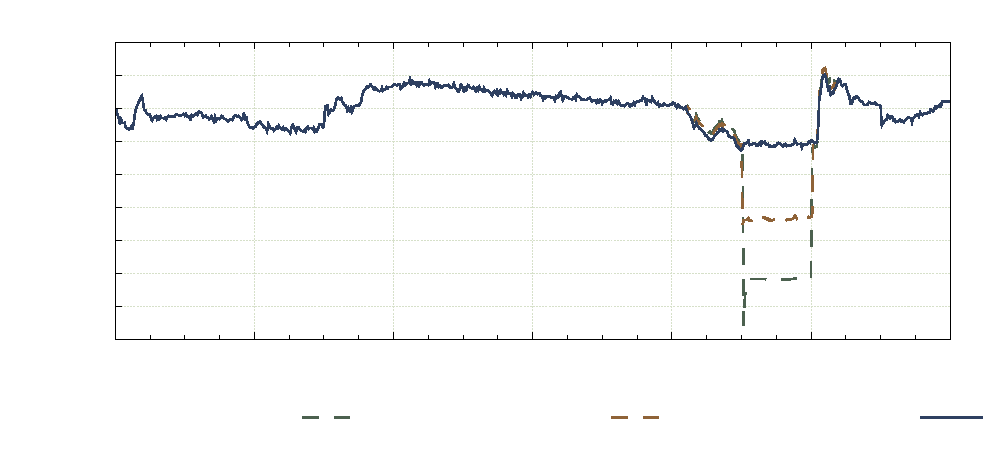
\includegraphics[trim=0 0 0.1cm 0, clip]{Graphs/4/KUSResults/StationFlow/Flow}}}%
    \gplfronttext
  \end{picture}%
\endgroup

		\caption{Flow reduction during blasting period for 105 level}
		\label{fig: 105 Flow savings}
	\end{figure}
Station control had the largest impact on the flow usage for the level. This result reflects the power reduction achieved by each intervention shown in \Cref{fig: Station vs stope}. The impact was 0.4 and 0.7 MW for the stope and station intervention respectively.
	
	\begin{figure}[h!]
		\centering
		% GNUPLOT: LaTeX picture with Postscript
\begingroup
  \makeatletter
  \providecommand\color[2][]{%
    \GenericError{(gnuplot) \space\space\space\@spaces}{%
      Package color not loaded in conjunction with
      terminal option `colourtext'%
    }{See the gnuplot documentation for explanation.%
    }{Either use 'blacktext' in gnuplot or load the package
      color.sty in LaTeX.}%
    \renewcommand\color[2][]{}%
  }%
  \providecommand\includegraphics[2][]{%
    \GenericError{(gnuplot) \space\space\space\@spaces}{%
      Package graphicx or graphics not loaded%
    }{See the gnuplot documentation for explanation.%
    }{The gnuplot epslatex terminal needs graphicx.sty or graphics.sty.}%
    \renewcommand\includegraphics[2][]{}%
  }%
  \providecommand\rotatebox[2]{#2}%
  \@ifundefined{ifGPcolor}{%
    \newif\ifGPcolor
    \GPcolortrue
  }{}%
  \@ifundefined{ifGPblacktext}{%
    \newif\ifGPblacktext
    \GPblacktextfalse
  }{}%
  % define a \g@addto@macro without @ in the name:
  \let\gplgaddtomacro\g@addto@macro
  % define empty templates for all commands taking text:
  \gdef\gplbacktext{}%
  \gdef\gplfronttext{}%
  \makeatother
  \ifGPblacktext
    % no textcolor at all
    \def\colorrgb#1{}%
    \def\colorgray#1{}%
  \else
    % gray or color?
    \ifGPcolor
      \def\colorrgb#1{\color[rgb]{#1}}%
      \def\colorgray#1{\color[gray]{#1}}%
      \expandafter\def\csname LTw\endcsname{\color{white}}%
      \expandafter\def\csname LTb\endcsname{\color{black}}%
      \expandafter\def\csname LTa\endcsname{\color{black}}%
      \expandafter\def\csname LT0\endcsname{\color[rgb]{1,0,0}}%
      \expandafter\def\csname LT1\endcsname{\color[rgb]{0,1,0}}%
      \expandafter\def\csname LT2\endcsname{\color[rgb]{0,0,1}}%
      \expandafter\def\csname LT3\endcsname{\color[rgb]{1,0,1}}%
      \expandafter\def\csname LT4\endcsname{\color[rgb]{0,1,1}}%
      \expandafter\def\csname LT5\endcsname{\color[rgb]{1,1,0}}%
      \expandafter\def\csname LT6\endcsname{\color[rgb]{0,0,0}}%
      \expandafter\def\csname LT7\endcsname{\color[rgb]{1,0.3,0}}%
      \expandafter\def\csname LT8\endcsname{\color[rgb]{0.5,0.5,0.5}}%
    \else
      % gray
      \def\colorrgb#1{\color{black}}%
      \def\colorgray#1{\color[gray]{#1}}%
      \expandafter\def\csname LTw\endcsname{\color{white}}%
      \expandafter\def\csname LTb\endcsname{\color{black}}%
      \expandafter\def\csname LTa\endcsname{\color{black}}%
      \expandafter\def\csname LT0\endcsname{\color{black}}%
      \expandafter\def\csname LT1\endcsname{\color{black}}%
      \expandafter\def\csname LT2\endcsname{\color{black}}%
      \expandafter\def\csname LT3\endcsname{\color{black}}%
      \expandafter\def\csname LT4\endcsname{\color{black}}%
      \expandafter\def\csname LT5\endcsname{\color{black}}%
      \expandafter\def\csname LT6\endcsname{\color{black}}%
      \expandafter\def\csname LT7\endcsname{\color{black}}%
      \expandafter\def\csname LT8\endcsname{\color{black}}%
    \fi
  \fi
    \setlength{\unitlength}{0.0500bp}%
    \ifx\gptboxheight\undefined%
      \newlength{\gptboxheight}%
      \newlength{\gptboxwidth}%
      \newsavebox{\gptboxtext}%
    \fi%
    \setlength{\fboxrule}{0.5pt}%
    \setlength{\fboxsep}{1pt}%
\begin{picture}(9360.00,4032.00)%
    \gplgaddtomacro\gplbacktext{%
      \colorrgb{0.00,0.00,0.00}%
      \put(682,1330){\makebox(0,0)[r]{\strut{}$8$}}%
      \colorrgb{0.00,0.00,0.00}%
      \put(682,2142){\makebox(0,0)[r]{\strut{}$10$}}%
      \colorrgb{0.00,0.00,0.00}%
      \put(682,2955){\makebox(0,0)[r]{\strut{}$12$}}%
      \colorrgb{0.00,0.00,0.00}%
      \put(682,3767){\makebox(0,0)[r]{\strut{}$14$}}%
      \colorrgb{0.00,0.00,0.00}%
      \put(814,704){\makebox(0,0){\strut{}00:00}}%
      \colorrgb{0.00,0.00,0.00}%
      \put(2172,704){\makebox(0,0){\strut{}04:00}}%
      \colorrgb{0.00,0.00,0.00}%
      \put(3530,704){\makebox(0,0){\strut{}08:00}}%
      \colorrgb{0.00,0.00,0.00}%
      \put(4888,704){\makebox(0,0){\strut{}12:00}}%
      \colorrgb{0.00,0.00,0.00}%
      \put(6246,704){\makebox(0,0){\strut{}16:00}}%
      \colorrgb{0.00,0.00,0.00}%
      \put(7604,704){\makebox(0,0){\strut{}20:00}}%
      \colorrgb{0.00,0.00,0.00}%
      \put(8962,704){\makebox(0,0){\strut{}00:00}}%
    }%
    \gplgaddtomacro\gplfronttext{%
      \csname LTb\endcsname%
      \put(176,2345){\rotatebox{-270}{\makebox(0,0){\strut{}Power $(MW)$}}}%
      \put(4888,374){\makebox(0,0){\strut{}Time of Day}}%
      \csname LTb\endcsname%
      \put(2549,173){\makebox(0,0)[r]{\strut{}Station control}}%
      \csname LTb\endcsname%
      \put(5516,173){\makebox(0,0)[r]{\strut{}In-stope control}}%
      \csname LTb\endcsname%
      \put(8483,173){\makebox(0,0)[r]{\strut{}Baseline}}%
    }%
    \gplbacktext
        \put(0,0){\fbox{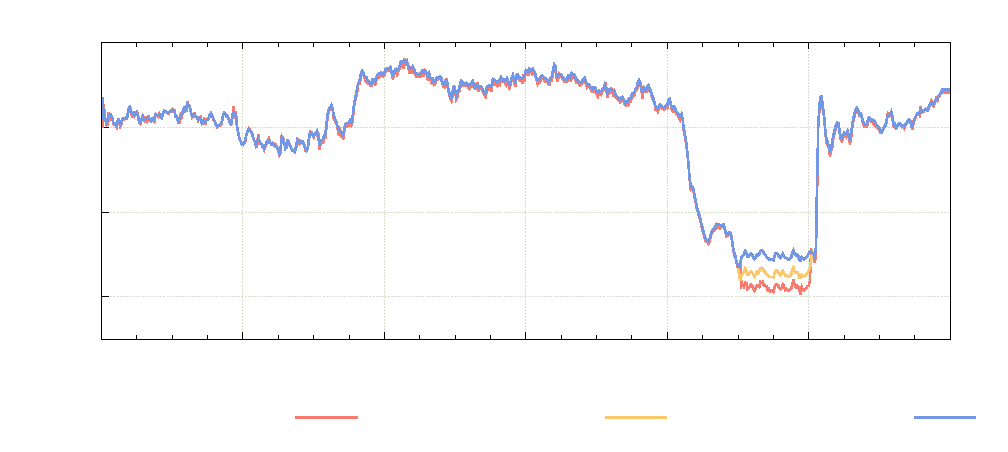
\includegraphics[trim=0 0 0.1cm 0, clip]{Graphs/4/KUSResults/StationPower/Station}}}%
    \gplfronttext
  \end{picture}%
\endgroup

		\caption{Comparing simulated flow interventions on 105L}
		\label{fig: Station vs stope}
	\end{figure}
A simulation was done to estimate the potential savings of extending the evening station control to other levels.  The flow demands for levels 95---115 were updated to match the flow saving achieved in the 105L simulation. The savings obtained in generalised station control simulation was 2.0 MW \gls{pc}, shown in \Cref{fig: General station optimise}. It was calculated that this would lead to an annual energy cost saving of R2.5M.
\begin{figure}[h!]
	\centering
	% GNUPLOT: LaTeX picture with Postscript
\begingroup
  \makeatletter
  \providecommand\color[2][]{%
    \GenericError{(gnuplot) \space\space\space\@spaces}{%
      Package color not loaded in conjunction with
      terminal option `colourtext'%
    }{See the gnuplot documentation for explanation.%
    }{Either use 'blacktext' in gnuplot or load the package
      color.sty in LaTeX.}%
    \renewcommand\color[2][]{}%
  }%
  \providecommand\includegraphics[2][]{%
    \GenericError{(gnuplot) \space\space\space\@spaces}{%
      Package graphicx or graphics not loaded%
    }{See the gnuplot documentation for explanation.%
    }{The gnuplot epslatex terminal needs graphicx.sty or graphics.sty.}%
    \renewcommand\includegraphics[2][]{}%
  }%
  \providecommand\rotatebox[2]{#2}%
  \@ifundefined{ifGPcolor}{%
    \newif\ifGPcolor
    \GPcolortrue
  }{}%
  \@ifundefined{ifGPblacktext}{%
    \newif\ifGPblacktext
    \GPblacktextfalse
  }{}%
  % define a \g@addto@macro without @ in the name:
  \let\gplgaddtomacro\g@addto@macro
  % define empty templates for all commands taking text:
  \gdef\gplbacktext{}%
  \gdef\gplfronttext{}%
  \makeatother
  \ifGPblacktext
    % no textcolor at all
    \def\colorrgb#1{}%
    \def\colorgray#1{}%
  \else
    % gray or color?
    \ifGPcolor
      \def\colorrgb#1{\color[rgb]{#1}}%
      \def\colorgray#1{\color[gray]{#1}}%
      \expandafter\def\csname LTw\endcsname{\color{white}}%
      \expandafter\def\csname LTb\endcsname{\color{black}}%
      \expandafter\def\csname LTa\endcsname{\color{black}}%
      \expandafter\def\csname LT0\endcsname{\color[rgb]{1,0,0}}%
      \expandafter\def\csname LT1\endcsname{\color[rgb]{0,1,0}}%
      \expandafter\def\csname LT2\endcsname{\color[rgb]{0,0,1}}%
      \expandafter\def\csname LT3\endcsname{\color[rgb]{1,0,1}}%
      \expandafter\def\csname LT4\endcsname{\color[rgb]{0,1,1}}%
      \expandafter\def\csname LT5\endcsname{\color[rgb]{1,1,0}}%
      \expandafter\def\csname LT6\endcsname{\color[rgb]{0,0,0}}%
      \expandafter\def\csname LT7\endcsname{\color[rgb]{1,0.3,0}}%
      \expandafter\def\csname LT8\endcsname{\color[rgb]{0.5,0.5,0.5}}%
    \else
      % gray
      \def\colorrgb#1{\color{black}}%
      \def\colorgray#1{\color[gray]{#1}}%
      \expandafter\def\csname LTw\endcsname{\color{white}}%
      \expandafter\def\csname LTb\endcsname{\color{black}}%
      \expandafter\def\csname LTa\endcsname{\color{black}}%
      \expandafter\def\csname LT0\endcsname{\color{black}}%
      \expandafter\def\csname LT1\endcsname{\color{black}}%
      \expandafter\def\csname LT2\endcsname{\color{black}}%
      \expandafter\def\csname LT3\endcsname{\color{black}}%
      \expandafter\def\csname LT4\endcsname{\color{black}}%
      \expandafter\def\csname LT5\endcsname{\color{black}}%
      \expandafter\def\csname LT6\endcsname{\color{black}}%
      \expandafter\def\csname LT7\endcsname{\color{black}}%
      \expandafter\def\csname LT8\endcsname{\color{black}}%
    \fi
  \fi
    \setlength{\unitlength}{0.0500bp}%
    \ifx\gptboxheight\undefined%
      \newlength{\gptboxheight}%
      \newlength{\gptboxwidth}%
      \newsavebox{\gptboxtext}%
    \fi%
    \setlength{\fboxrule}{0.5pt}%
    \setlength{\fboxsep}{1pt}%
\begin{picture}(9360.00,4032.00)%
    \gplgaddtomacro\gplbacktext{%
      \colorrgb{0.00,0.00,0.00}%
      \put(682,924){\makebox(0,0)[r]{\strut{}$0$}}%
      \colorrgb{0.00,0.00,0.00}%
      \put(682,1736){\makebox(0,0)[r]{\strut{}$4$}}%
      \colorrgb{0.00,0.00,0.00}%
      \put(682,2549){\makebox(0,0)[r]{\strut{}$8$}}%
      \colorrgb{0.00,0.00,0.00}%
      \put(682,3361){\makebox(0,0)[r]{\strut{}$12$}}%
      \colorrgb{0.00,0.00,0.00}%
      \put(814,704){\makebox(0,0){\strut{}00:00}}%
      \colorrgb{0.00,0.00,0.00}%
      \put(2172,704){\makebox(0,0){\strut{}04:00}}%
      \colorrgb{0.00,0.00,0.00}%
      \put(3530,704){\makebox(0,0){\strut{}08:00}}%
      \colorrgb{0.00,0.00,0.00}%
      \put(4888,704){\makebox(0,0){\strut{}12:00}}%
      \colorrgb{0.00,0.00,0.00}%
      \put(6246,704){\makebox(0,0){\strut{}16:00}}%
      \colorrgb{0.00,0.00,0.00}%
      \put(7604,704){\makebox(0,0){\strut{}20:00}}%
      \colorrgb{0.00,0.00,0.00}%
      \put(8962,704){\makebox(0,0){\strut{}00:00}}%
    }%
    \gplgaddtomacro\gplfronttext{%
      \csname LTb\endcsname%
      \put(176,2345){\rotatebox{-270}{\makebox(0,0){\strut{}Power $(MW)$}}}%
      \put(4888,374){\makebox(0,0){\strut{}Time of day}}%
      \csname LTb\endcsname%
      \put(2747,173){\makebox(0,0)[r]{\strut{}Intervention}}%
      \csname LTb\endcsname%
      \put(5318,173){\makebox(0,0)[r]{\strut{}Power Savings}}%
      \csname LTb\endcsname%
      \put(7889,173){\makebox(0,0)[r]{\strut{}Baseline}}%
    }%
    \gplbacktext
    \put(0,0){\fbox{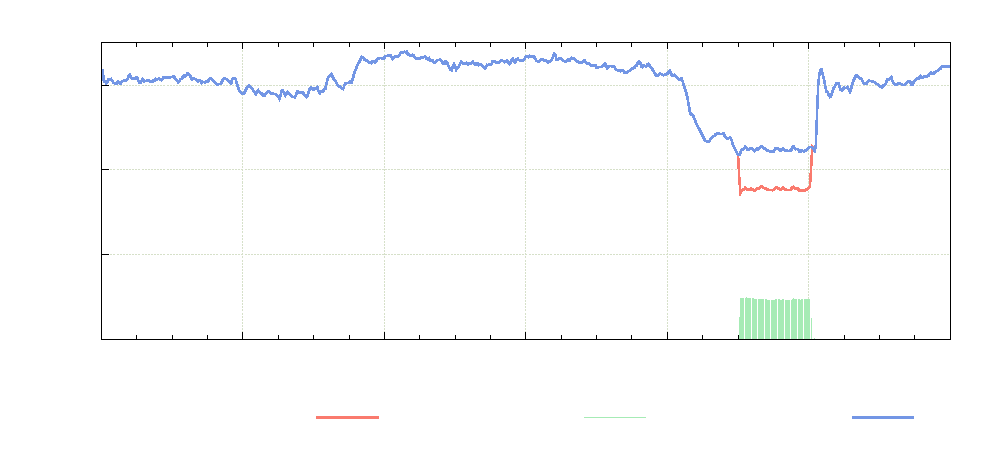
\includegraphics[trim=0 0 0.1cm 0, clip]{Graphs/4/KUSResults/General/Power}}}%
    \gplfronttext
  \end{picture}%
\endgroup

	\caption{Energy saving achieved by general peak time station control }
	\label{fig: General station optimise}
\end{figure}
	\subsection{Comparison of interventions}
	The interventions were then compared to feedback to the mine. The refuge bay intervention is recommended as it will achieve the highest energy cost saving. These results were used to produce a report that was sent to the responsible personnel at Mine B.
	\begin{table}[h!]
		\centering
		\begin{tabular}{p{0.45\textwidth-2\tabcolsep - 1.25\arrayrulewidth}
				p{0.2\textwidth-2\tabcolsep - 1.25\arrayrulewidth}
				p{0.1\textwidth-2\tabcolsep - 1.25\arrayrulewidth}
				p{0.25\textwidth-2\tabcolsep - 1.25\arrayrulewidth}}
			\hline 
			 \vspace{0.5em}Scenario & \vspace{0.5em}Power saving & Cost saving (\gls{pa}) & \vspace{0.5em}Additional benefit \\
			\hline
			\multicolumn{4}{l}{\textbf{Scenario 1 results}} \\
			Refuge bay leakage reduction & $ 0.92 $ MW \gls{ee} & R5.17M & Increase in drilling pressure \\
			 \\
			\multicolumn{4}{l}{\textbf{Scenario 2 results}} \\
			105L peak time in-Stope control & $ 0.4 $ MW \gls{pc} & R$ 0.3 $M& - \\
			105L peak time Station control & $ 0.7 $ MW \gls{pc} & R$ 2.5 $M& - \\
			General peak time Station control & $ 2.0 $ MW \gls{pc} & R$ 2.5 $M& - \\
			\hline 
		\end{tabular}
		\caption{Comparison of the simulated scenarios}
		\label{Table: B Comparison}
	\end{table}
	%\subsection{Validation of results}
%	- Awaiting results on manual tests
%	- 
	\subsection{Summary}
	A second case study was implemented on a mine compressed air network. An investigation was performed to gather data and identify potential interventions. This investigation included underground spot checks and measurements.
	\par 
	 A simulation model was developed to test scenarios. Two scenarios (refuge bay optimisations and per level flow optimisations) were simulated. The simulated interventions showed an \gls{ee} saving of up to 0.92 MW which would result in a cost saving of R5.17M with an additional pressure improvement for scenario 1. The results for scenario 2 showed a \gls{pc} impact of up to 2 MW with an annual energy cost saving of R2.5M. The results of the simulations were reported to the mine.
\section{Case study 3: Periodic simulation analysis}
	\subsection{Preamble}
	Periodically updating the inputs of a simulation could be used to verify the compressed air model accuracy. If the precision of simulation outputs remains within constraints for subsequent days, this would indicate that the model is correctly calibrated. Additionally, this process could be used to identify significant operational changes that occur within the system. The operational changes would cause the simulation outputs to differ from the actual measured parameters. This information can be used to make improvements to the system.
	\par 
	A daily periodic simulation analysis was implemented between 2016/11/01 and 2016/11/30 using the periodic simulation methodology discussed in Chapter 3. The simulation model developed for case study A was used for the analysis. The simulation receives the data inputs shown in \Cref{table: Periodic inputs/outputs}.
	\begin{table}[h!]
		\centering
		\begin{tabular}{ll}
			\hline
			Inputs \hspace*{4cm} &Outputs \hspace*{4cm} \\ \hhline{==}
			Ambient air conditions&Compressor power \\
			Measured flows& Flows \\
			Compressor schedules& Pressures \\
			\hline
		\end{tabular}
		\caption{Data inputs and outputs for the simulation}
		\label{table: Periodic inputs/outputs}
	\end{table}

\subsection{Results}

 The process was triggered daily. For each period, data inputs shown in \Cref{table: Periodic inputs/outputs} were imported into the model, the simulation was then processed, and the outputs are compared with the real system parameters. \Cref{fig: Periodic simulation} shows the average daily accuracy of the simulated total system power, flow and the shaft pressure per period.
	 \par 
 
	\begin{figure}[h!]
		\centering
		% GNUPLOT: LaTeX picture with Postscript
\begingroup
  \makeatletter
  \providecommand\color[2][]{%
    \GenericError{(gnuplot) \space\space\space\@spaces}{%
      Package color not loaded in conjunction with
      terminal option `colourtext'%
    }{See the gnuplot documentation for explanation.%
    }{Either use 'blacktext' in gnuplot or load the package
      color.sty in LaTeX.}%
    \renewcommand\color[2][]{}%
  }%
  \providecommand\includegraphics[2][]{%
    \GenericError{(gnuplot) \space\space\space\@spaces}{%
      Package graphicx or graphics not loaded%
    }{See the gnuplot documentation for explanation.%
    }{The gnuplot epslatex terminal needs graphicx.sty or graphics.sty.}%
    \renewcommand\includegraphics[2][]{}%
  }%
  \providecommand\rotatebox[2]{#2}%
  \@ifundefined{ifGPcolor}{%
    \newif\ifGPcolor
    \GPcolortrue
  }{}%
  \@ifundefined{ifGPblacktext}{%
    \newif\ifGPblacktext
    \GPblacktextfalse
  }{}%
  % define a \g@addto@macro without @ in the name:
  \let\gplgaddtomacro\g@addto@macro
  % define empty templates for all commands taking text:
  \gdef\gplbacktext{}%
  \gdef\gplfronttext{}%
  \makeatother
  \ifGPblacktext
    % no textcolor at all
    \def\colorrgb#1{}%
    \def\colorgray#1{}%
  \else
    % gray or color?
    \ifGPcolor
      \def\colorrgb#1{\color[rgb]{#1}}%
      \def\colorgray#1{\color[gray]{#1}}%
      \expandafter\def\csname LTw\endcsname{\color{white}}%
      \expandafter\def\csname LTb\endcsname{\color{black}}%
      \expandafter\def\csname LTa\endcsname{\color{black}}%
      \expandafter\def\csname LT0\endcsname{\color[rgb]{1,0,0}}%
      \expandafter\def\csname LT1\endcsname{\color[rgb]{0,1,0}}%
      \expandafter\def\csname LT2\endcsname{\color[rgb]{0,0,1}}%
      \expandafter\def\csname LT3\endcsname{\color[rgb]{1,0,1}}%
      \expandafter\def\csname LT4\endcsname{\color[rgb]{0,1,1}}%
      \expandafter\def\csname LT5\endcsname{\color[rgb]{1,1,0}}%
      \expandafter\def\csname LT6\endcsname{\color[rgb]{0,0,0}}%
      \expandafter\def\csname LT7\endcsname{\color[rgb]{1,0.3,0}}%
      \expandafter\def\csname LT8\endcsname{\color[rgb]{0.5,0.5,0.5}}%
    \else
      % gray
      \def\colorrgb#1{\color{black}}%
      \def\colorgray#1{\color[gray]{#1}}%
      \expandafter\def\csname LTw\endcsname{\color{white}}%
      \expandafter\def\csname LTb\endcsname{\color{black}}%
      \expandafter\def\csname LTa\endcsname{\color{black}}%
      \expandafter\def\csname LT0\endcsname{\color{black}}%
      \expandafter\def\csname LT1\endcsname{\color{black}}%
      \expandafter\def\csname LT2\endcsname{\color{black}}%
      \expandafter\def\csname LT3\endcsname{\color{black}}%
      \expandafter\def\csname LT4\endcsname{\color{black}}%
      \expandafter\def\csname LT5\endcsname{\color{black}}%
      \expandafter\def\csname LT6\endcsname{\color{black}}%
      \expandafter\def\csname LT7\endcsname{\color{black}}%
      \expandafter\def\csname LT8\endcsname{\color{black}}%
    \fi
  \fi
    \setlength{\unitlength}{0.0500bp}%
    \ifx\gptboxheight\undefined%
      \newlength{\gptboxheight}%
      \newlength{\gptboxwidth}%
      \newsavebox{\gptboxtext}%
    \fi%
    \setlength{\fboxrule}{0.5pt}%
    \setlength{\fboxsep}{1pt}%
\begin{picture}(9360.00,4032.00)%
    \gplgaddtomacro\gplbacktext{%
      \colorrgb{0.00,0.00,0.00}%
      \put(814,924){\makebox(0,0)[r]{\strut{}$80$}}%
      \colorrgb{0.00,0.00,0.00}%
      \put(814,1635){\makebox(0,0)[r]{\strut{}$85$}}%
      \colorrgb{0.00,0.00,0.00}%
      \put(814,2346){\makebox(0,0)[r]{\strut{}$90$}}%
      \colorrgb{0.00,0.00,0.00}%
      \put(814,3056){\makebox(0,0)[r]{\strut{}$95$}}%
      \colorrgb{0.00,0.00,0.00}%
      \put(814,3767){\makebox(0,0)[r]{\strut{}$100$}}%
      \colorrgb{0.00,0.00,0.00}%
      \put(946,704){\makebox(0,0){\strut{}2016/11/01}}%
      \colorrgb{0.00,0.00,0.00}%
      \put(2604,704){\makebox(0,0){\strut{}2016/11/07}}%
      \colorrgb{0.00,0.00,0.00}%
      \put(4263,704){\makebox(0,0){\strut{}2016/11/13}}%
      \colorrgb{0.00,0.00,0.00}%
      \put(5921,704){\makebox(0,0){\strut{}2016/11/19}}%
      \colorrgb{0.00,0.00,0.00}%
      \put(7580,704){\makebox(0,0){\strut{}2016/11/25}}%
    }%
    \gplgaddtomacro\gplfronttext{%
      \csname LTb\endcsname%
      \put(176,2345){\rotatebox{-270}{\makebox(0,0){\strut{}Accuracy (\%)}}}%
      \put(4954,374){\makebox(0,0){\strut{}Date of simulation}}%
      \csname LTb\endcsname%
      \put(3143,173){\makebox(0,0)[r]{\strut{}Flow}}%
      \csname LTb\endcsname%
      \put(5054,173){\makebox(0,0)[r]{\strut{}Pressure}}%
      \csname LTb\endcsname%
      \put(6965,173){\makebox(0,0)[r]{\strut{}Power}}%
    }%
    \gplbacktext
    \put(0,0){\fbox{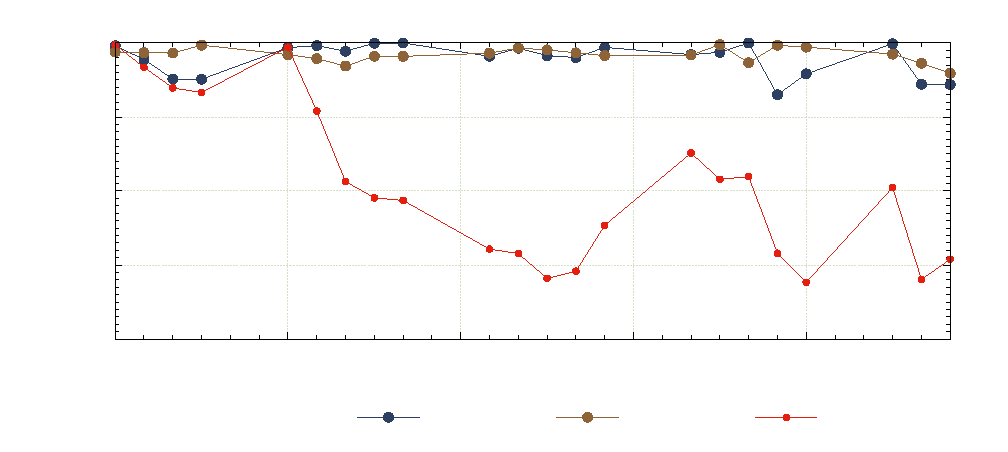
\includegraphics[trim=0 0 0.1cm 0, clip]{Graphs/4/Periodic1/Periodic1}}}%
    \gplfronttext
  \end{picture}%
\endgroup

		\caption{The flow, pressure and power error percentages for daily periodic simulations over a month}
		\label{fig: Periodic simulation}
	\end{figure} 
The accuracy of the process parameters of the simulation was within 5\% for the duration of the periodic simulation. However, From the 2016/11/07, the accuracy of the simulated power dropped by between 10 and 15 percent. The average daily power of the system up to that point was approximately 12.5 MW. A 15\% simulation error then relates to 1.9 MW difference between simulated and actual values. This error suggests a major shift in operation of the system.
\par 
An analysis was done to try to determine the source of the discrepancy. From the data, it was identified that the simulated power for compressor 1 was the source of the different A look at the actual power measurement for compressor one show drop compared to normal operation by almost 2 MW. At the same time, the power used per kg/s of air seemed to have dropped. \Cref{fig: MeasurementAccuracy.} shows the average daily power for compressor 1 (blue), compared to the air mass flow per Watt(yellow). 
\par
	\begin{figure}[h!]
		\centering
		% GNUPLOT: LaTeX picture with Postscript
\begingroup
  \makeatletter
  \providecommand\color[2][]{%
    \GenericError{(gnuplot) \space\space\space\@spaces}{%
      Package color not loaded in conjunction with
      terminal option `colourtext'%
    }{See the gnuplot documentation for explanation.%
    }{Either use 'blacktext' in gnuplot or load the package
      color.sty in LaTeX.}%
    \renewcommand\color[2][]{}%
  }%
  \providecommand\includegraphics[2][]{%
    \GenericError{(gnuplot) \space\space\space\@spaces}{%
      Package graphicx or graphics not loaded%
    }{See the gnuplot documentation for explanation.%
    }{The gnuplot epslatex terminal needs graphicx.sty or graphics.sty.}%
    \renewcommand\includegraphics[2][]{}%
  }%
  \providecommand\rotatebox[2]{#2}%
  \@ifundefined{ifGPcolor}{%
    \newif\ifGPcolor
    \GPcolortrue
  }{}%
  \@ifundefined{ifGPblacktext}{%
    \newif\ifGPblacktext
    \GPblacktextfalse
  }{}%
  % define a \g@addto@macro without @ in the name:
  \let\gplgaddtomacro\g@addto@macro
  % define empty templates for all commands taking text:
  \gdef\gplbacktext{}%
  \gdef\gplfronttext{}%
  \makeatother
  \ifGPblacktext
    % no textcolor at all
    \def\colorrgb#1{}%
    \def\colorgray#1{}%
  \else
    % gray or color?
    \ifGPcolor
      \def\colorrgb#1{\color[rgb]{#1}}%
      \def\colorgray#1{\color[gray]{#1}}%
      \expandafter\def\csname LTw\endcsname{\color{white}}%
      \expandafter\def\csname LTb\endcsname{\color{black}}%
      \expandafter\def\csname LTa\endcsname{\color{black}}%
      \expandafter\def\csname LT0\endcsname{\color[rgb]{1,0,0}}%
      \expandafter\def\csname LT1\endcsname{\color[rgb]{0,1,0}}%
      \expandafter\def\csname LT2\endcsname{\color[rgb]{0,0,1}}%
      \expandafter\def\csname LT3\endcsname{\color[rgb]{1,0,1}}%
      \expandafter\def\csname LT4\endcsname{\color[rgb]{0,1,1}}%
      \expandafter\def\csname LT5\endcsname{\color[rgb]{1,1,0}}%
      \expandafter\def\csname LT6\endcsname{\color[rgb]{0,0,0}}%
      \expandafter\def\csname LT7\endcsname{\color[rgb]{1,0.3,0}}%
      \expandafter\def\csname LT8\endcsname{\color[rgb]{0.5,0.5,0.5}}%
    \else
      % gray
      \def\colorrgb#1{\color{black}}%
      \def\colorgray#1{\color[gray]{#1}}%
      \expandafter\def\csname LTw\endcsname{\color{white}}%
      \expandafter\def\csname LTb\endcsname{\color{black}}%
      \expandafter\def\csname LTa\endcsname{\color{black}}%
      \expandafter\def\csname LT0\endcsname{\color{black}}%
      \expandafter\def\csname LT1\endcsname{\color{black}}%
      \expandafter\def\csname LT2\endcsname{\color{black}}%
      \expandafter\def\csname LT3\endcsname{\color{black}}%
      \expandafter\def\csname LT4\endcsname{\color{black}}%
      \expandafter\def\csname LT5\endcsname{\color{black}}%
      \expandafter\def\csname LT6\endcsname{\color{black}}%
      \expandafter\def\csname LT7\endcsname{\color{black}}%
      \expandafter\def\csname LT8\endcsname{\color{black}}%
    \fi
  \fi
    \setlength{\unitlength}{0.0500bp}%
    \ifx\gptboxheight\undefined%
      \newlength{\gptboxheight}%
      \newlength{\gptboxwidth}%
      \newsavebox{\gptboxtext}%
    \fi%
    \setlength{\fboxrule}{0.5pt}%
    \setlength{\fboxsep}{1pt}%
\begin{picture}(9360.00,3528.00)%
    \gplgaddtomacro\gplbacktext{%
      \colorrgb{0.00,0.00,0.00}%
      \put(946,924){\makebox(0,0)[r]{\strut{}$1000$}}%
      \colorrgb{0.00,0.00,0.00}%
      \put(946,1314){\makebox(0,0)[r]{\strut{}$1500$}}%
      \colorrgb{0.00,0.00,0.00}%
      \put(946,1704){\makebox(0,0)[r]{\strut{}$2000$}}%
      \colorrgb{0.00,0.00,0.00}%
      \put(946,2094){\makebox(0,0)[r]{\strut{}$2500$}}%
      \colorrgb{0.00,0.00,0.00}%
      \put(946,2483){\makebox(0,0)[r]{\strut{}$3000$}}%
      \colorrgb{0.00,0.00,0.00}%
      \put(946,2873){\makebox(0,0)[r]{\strut{}$3500$}}%
      \colorrgb{0.00,0.00,0.00}%
      \put(946,3263){\makebox(0,0)[r]{\strut{}$4000$}}%
      \colorrgb{0.00,0.00,0.00}%
      \put(1078,704){\makebox(0,0){\strut{}2016/09/01}}%
      \colorrgb{0.00,0.00,0.00}%
      \put(3118,704){\makebox(0,0){\strut{}2016/10/01}}%
      \colorrgb{0.00,0.00,0.00}%
      \put(5226,704){\makebox(0,0){\strut{}2016/11/01}}%
      \colorrgb{0.00,0.00,0.00}%
      \put(5226,704){\makebox(0,0){\strut{}2016/11/01}}%
      \colorrgb{0.00,0.00,0.00}%
      \put(7266,704){\makebox(0,0){\strut{}2016/12/01}}%
      \colorrgb{0.00,0.00,0.00}%
      \put(8214,924){\makebox(0,0)[l]{\strut{}$2$}}%
      \colorrgb{0.00,0.00,0.00}%
      \put(8214,1314){\makebox(0,0)[l]{\strut{}$2.5$}}%
      \colorrgb{0.00,0.00,0.00}%
      \put(8214,1704){\makebox(0,0)[l]{\strut{}$3$}}%
      \colorrgb{0.00,0.00,0.00}%
      \put(8214,2094){\makebox(0,0)[l]{\strut{}$3.5$}}%
      \colorrgb{0.00,0.00,0.00}%
      \put(8214,2483){\makebox(0,0)[l]{\strut{}$4$}}%
      \colorrgb{0.00,0.00,0.00}%
      \put(8214,2873){\makebox(0,0)[l]{\strut{}$4.5$}}%
      \colorrgb{0.00,0.00,0.00}%
      \put(8214,3263){\makebox(0,0)[l]{\strut{}$5$}}%
    }%
    \gplgaddtomacro\gplfronttext{%
      \csname LTb\endcsname%
      \put(176,2093){\rotatebox{-270}{\makebox(0,0){\strut{}Power (kW)}}}%
      \put(8851,2093){\rotatebox{-270}{\makebox(0,0){\strut{}$Flow per Watt (kg/s/W)$}}}%
      \put(4580,374){\makebox(0,0){\strut{}Date}}%
      \csname LTb\endcsname%
      \put(3725,173){\makebox(0,0)[r]{\strut{}Compressor 1 average power}}%
      \csname LTb\endcsname%
      \put(8012,173){\makebox(0,0)[r]{\strut{}System efficiency}}%
      \csname LTb\endcsname%
      \put(6220,3029){\makebox(0,0){\strut{}\shortstack{\small{Periodic simulation}}}}%
    }%
    \gplbacktext
    \put(0,0){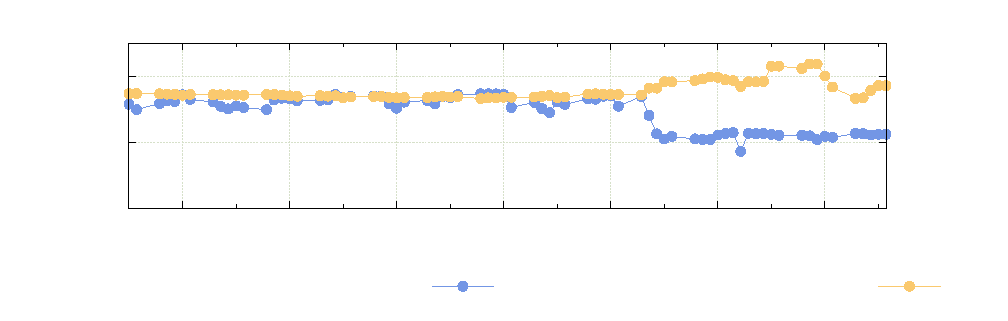
\includegraphics{Graphs/4/PeriodicRange/PeriodicRange}}%
    \gplfronttext
  \end{picture}%
\endgroup

		\caption{Supply efficiency and compressor 1's average power output over the time of the periodic analysis}
		\label{fig: MeasurementAccuracy.}
	\end{figure} 

A 2 MW shift in power is not likely; the results likely indicate that there was a fault in the power metering starting from 2016/11/07. A measurement error explains the perceived increase in efficiency over the same period as less power is measure then is being provided.  In this situation, the simulated power measurement is a more accurate metric for compressor 1’s power over this period.
 \subsection{Validation}
To validation of misreadings from the power meter from comparing independent power data for the substation to the combined individual compressors meters.\Cref{fig: Corrected Periodic simulation} shows the measured power from the two sources. By comparing the compressor power to the independent data, it is clear that there is an error in measurement as hypothesised.
	\begin{figure}[h!]
		\centering
		% GNUPLOT: LaTeX picture with Postscript
\begingroup
  \makeatletter
  \providecommand\color[2][]{%
    \GenericError{(gnuplot) \space\space\space\@spaces}{%
      Package color not loaded in conjunction with
      terminal option `colourtext'%
    }{See the gnuplot documentation for explanation.%
    }{Either use 'blacktext' in gnuplot or load the package
      color.sty in LaTeX.}%
    \renewcommand\color[2][]{}%
  }%
  \providecommand\includegraphics[2][]{%
    \GenericError{(gnuplot) \space\space\space\@spaces}{%
      Package graphicx or graphics not loaded%
    }{See the gnuplot documentation for explanation.%
    }{The gnuplot epslatex terminal needs graphicx.sty or graphics.sty.}%
    \renewcommand\includegraphics[2][]{}%
  }%
  \providecommand\rotatebox[2]{#2}%
  \@ifundefined{ifGPcolor}{%
    \newif\ifGPcolor
    \GPcolortrue
  }{}%
  \@ifundefined{ifGPblacktext}{%
    \newif\ifGPblacktext
    \GPblacktextfalse
  }{}%
  % define a \g@addto@macro without @ in the name:
  \let\gplgaddtomacro\g@addto@macro
  % define empty templates for all commands taking text:
  \gdef\gplbacktext{}%
  \gdef\gplfronttext{}%
  \makeatother
  \ifGPblacktext
    % no textcolor at all
    \def\colorrgb#1{}%
    \def\colorgray#1{}%
  \else
    % gray or color?
    \ifGPcolor
      \def\colorrgb#1{\color[rgb]{#1}}%
      \def\colorgray#1{\color[gray]{#1}}%
      \expandafter\def\csname LTw\endcsname{\color{white}}%
      \expandafter\def\csname LTb\endcsname{\color{black}}%
      \expandafter\def\csname LTa\endcsname{\color{black}}%
      \expandafter\def\csname LT0\endcsname{\color[rgb]{1,0,0}}%
      \expandafter\def\csname LT1\endcsname{\color[rgb]{0,1,0}}%
      \expandafter\def\csname LT2\endcsname{\color[rgb]{0,0,1}}%
      \expandafter\def\csname LT3\endcsname{\color[rgb]{1,0,1}}%
      \expandafter\def\csname LT4\endcsname{\color[rgb]{0,1,1}}%
      \expandafter\def\csname LT5\endcsname{\color[rgb]{1,1,0}}%
      \expandafter\def\csname LT6\endcsname{\color[rgb]{0,0,0}}%
      \expandafter\def\csname LT7\endcsname{\color[rgb]{1,0.3,0}}%
      \expandafter\def\csname LT8\endcsname{\color[rgb]{0.5,0.5,0.5}}%
    \else
      % gray
      \def\colorrgb#1{\color{black}}%
      \def\colorgray#1{\color[gray]{#1}}%
      \expandafter\def\csname LTw\endcsname{\color{white}}%
      \expandafter\def\csname LTb\endcsname{\color{black}}%
      \expandafter\def\csname LTa\endcsname{\color{black}}%
      \expandafter\def\csname LT0\endcsname{\color{black}}%
      \expandafter\def\csname LT1\endcsname{\color{black}}%
      \expandafter\def\csname LT2\endcsname{\color{black}}%
      \expandafter\def\csname LT3\endcsname{\color{black}}%
      \expandafter\def\csname LT4\endcsname{\color{black}}%
      \expandafter\def\csname LT5\endcsname{\color{black}}%
      \expandafter\def\csname LT6\endcsname{\color{black}}%
      \expandafter\def\csname LT7\endcsname{\color{black}}%
      \expandafter\def\csname LT8\endcsname{\color{black}}%
    \fi
  \fi
    \setlength{\unitlength}{0.0500bp}%
    \ifx\gptboxheight\undefined%
      \newlength{\gptboxheight}%
      \newlength{\gptboxwidth}%
      \newsavebox{\gptboxtext}%
    \fi%
    \setlength{\fboxrule}{0.5pt}%
    \setlength{\fboxsep}{1pt}%
\begin{picture}(9360.00,4284.00)%
    \gplgaddtomacro\gplbacktext{%
      \colorrgb{0.00,0.00,0.00}%
      \put(682,1366){\makebox(0,0)[r]{\strut{}$8$}}%
      \colorrgb{0.00,0.00,0.00}%
      \put(682,2250){\makebox(0,0)[r]{\strut{}$10$}}%
      \colorrgb{0.00,0.00,0.00}%
      \put(682,3135){\makebox(0,0)[r]{\strut{}$12$}}%
      \colorrgb{0.00,0.00,0.00}%
      \put(682,4019){\makebox(0,0)[r]{\strut{}$14$}}%
      \colorrgb{0.00,0.00,0.00}%
      \put(1938,704){\makebox(0,0){\strut{}05/11/2016}}%
      \colorrgb{0.00,0.00,0.00}%
      \put(3343,704){\makebox(0,0){\strut{}10/11/2016}}%
      \colorrgb{0.00,0.00,0.00}%
      \put(4748,704){\makebox(0,0){\strut{}15/11/2016}}%
      \colorrgb{0.00,0.00,0.00}%
      \put(6152,704){\makebox(0,0){\strut{}20/11/2016}}%
      \colorrgb{0.00,0.00,0.00}%
      \put(7557,704){\makebox(0,0){\strut{}25/11/2016}}%
      \colorrgb{0.00,0.00,0.00}%
      \put(8962,704){\makebox(0,0){\strut{}30/11/2016}}%
    }%
    \gplgaddtomacro\gplfronttext{%
      \csname LTb\endcsname%
      \put(176,2471){\rotatebox{-270}{\makebox(0,0){\strut{}Power (MW)}}}%
      \put(4888,374){\makebox(0,0){\strut{}Date}}%
      \csname LTb\endcsname%
      \put(4033,173){\makebox(0,0)[r]{\strut{}Compressor power measrement}}%
      \csname LTb\endcsname%
      \put(8452,173){\makebox(0,0)[r]{\strut{}Independant measurement}}%
    }%
    \gplbacktext
    \put(0,0){\fbox{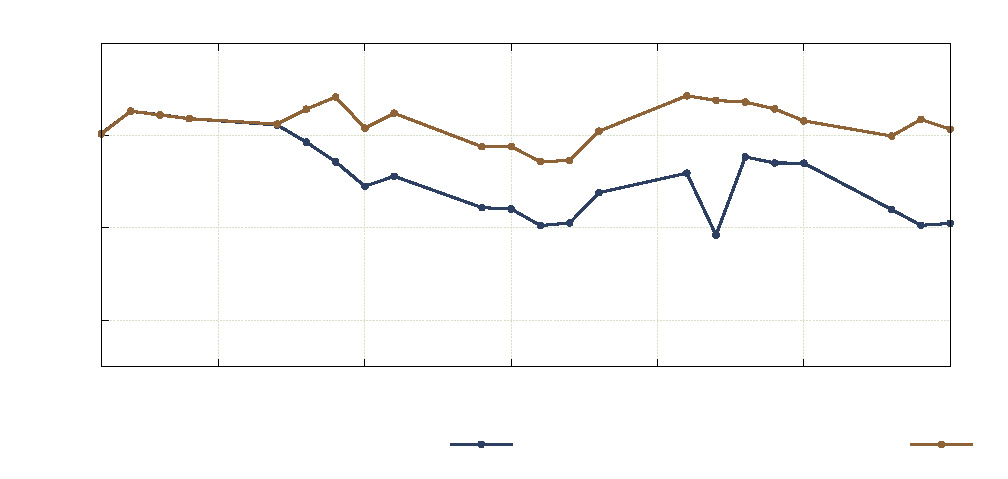
\includegraphics[trim=0 0 0.1cm 0, clip]{Graphs/4/PeriodicValidation/PeriodicValidation}}}%
    \gplfronttext
  \end{picture}%
\endgroup

		\caption{Comparison using alternative power source.}
		\label{fig: Corrected Periodic simulation}
	\end{figure} 
	
	\subsection{Summary}
	An investigation into periodic or repeated simulation was performed. Using the simulation model for Mine B, the periodic simulation methodology was implemented. The results indicated that the model was valid for consecutive days in the test range and identified an error in power measurement. Further analysis is recommended to determine how long a simulation model can remain valid before calibration is required.
\section{Potential benefit for SA mines}
There are approximately 75 operational gold and \gls{pgm} mines in South Africa, as illustrated in \Cref{fig: Mine map} \footnote{ Chamber of Mines, [Online] \url{http://www.chamberofmines.org.za/sa-mining/gold}, [Accessed 16-06-2017]}$^,$\footnote{ Chamber of Mines, [Online] \url{http://www.chamberofmines.org.za/sa-mining/platinum}, [Accessed 16-06-2017]}. Each mine utilises compressed air for underground processes. By utilising the compressed air simulation methodology in this study, the mines could collectively achieve significant energy and cost savings for the industry. 
\par 
	\begin{figure}[h!]
		\centering
		\fbox{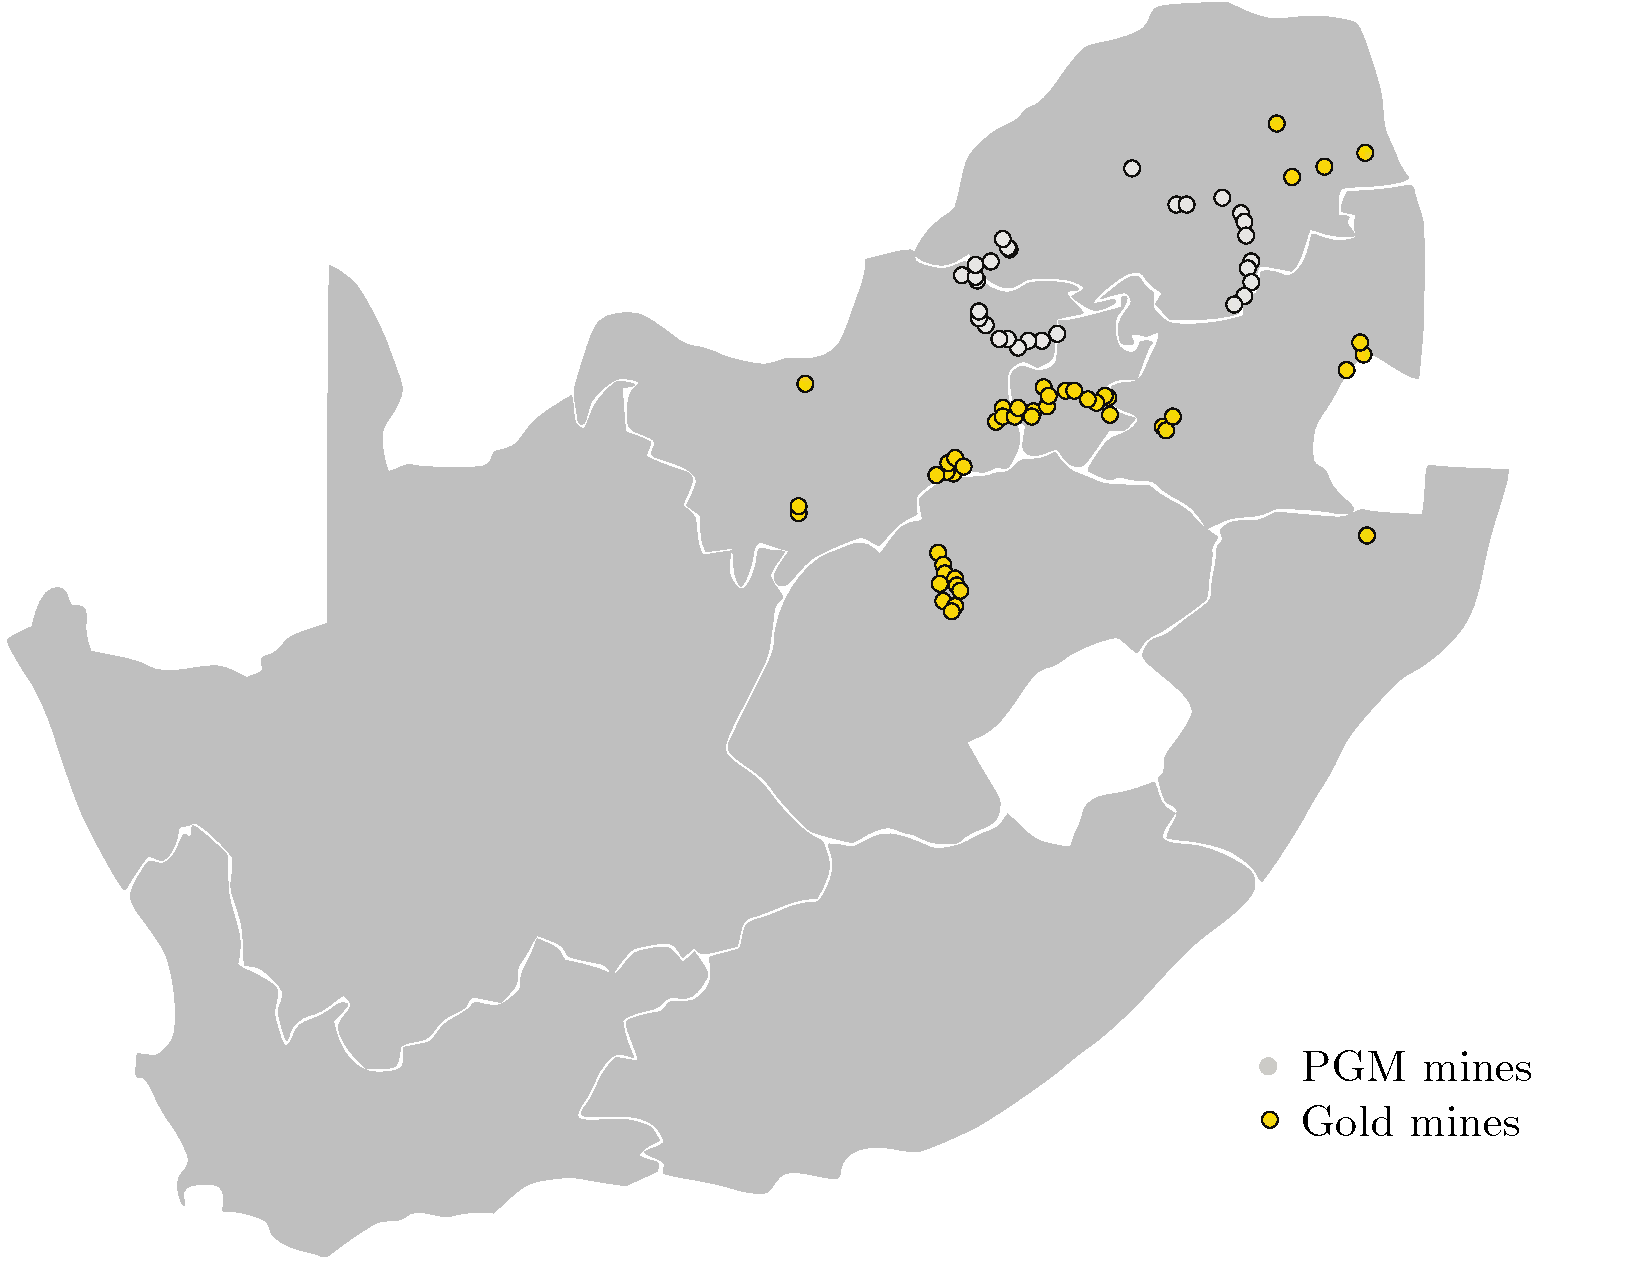
\includegraphics[width=0.85\textwidth]{Images/4/Mines3_optimized}}
		\caption[Gold and Platinum group metal mines in South Africa]{Gold and \gls{pgm} mines in South Africa$^{1,2}$}
		\label{fig: Mine map}
	\end{figure}
In this study, the simulated interventions resulted in savings of (on average) 0.69 MW \gls{ee} or 1.025 $ MW $ \gls{pc}. Assuming similar intervention were identified, through simulation for all gold and platinum mines. A potential energy saving of approximately 50 MW \gls{ee} or 75 $ MW $ \gls{pc} could be achieved. The combined cost saving for these interventions would amount to up to R400M \gls{pa}.
\clearpage
\section{Conclusion}
Chapter 4 aimed to validate the methodology developed in Chapter 3. This validation was achieved through the implementation of two case studies South African gold mines. A third case study was performed to analyse and validate the value repeated/periodic simulation.
\par 
In case study 1, the compressed air network for gold mining complex consisting of three mining shafts was investigated. A simulation model was then developed, and the accuracy was verified using typical operation from historical data. Two scenarios were simulated, Optimising compressor set-points and reducing pressure during the evening energy peak.
\par 
The results showed that there was a potential P.C. power reduction of 0.46 and 1.0 MW respectively. The reduction in power during the energy peak times could lead to a potential cost reduction of up to R0.91M. The result was validated using results of actual tests on the system.
\par
In case study 2, the same procedure was applied to another gold mine.  The mine consisted of a main and sub-shaft. An investigation was done to gather data and identify potential interventions. The investigation included underground spot checks and measurements.
\par 
A simulation model was developed for the system. Two scenarios were simulated using the developed model. The simulations showed an \gls{ee} saving of up to 0.92 MW for scenario 1 and a \gls{pc} impact of up to 2 MW for scenario 2. The intervention could lead to an energy cost saving of R5.17M for the mine. Additional pressure improvements were identified in case study 1. The results were reported to the mine.
\par
A third case study was performed to validate the periodic or repeated simulation methodology. The results showed that the simulation model remained valid for consecutive days in the tested date range. Faulty power measurements were also identified from the results. Further analysis was recommended to determine how long a simulation model can remain valid before calibration is required.
\par 
Finally, the result of large-scale implementation of compressed air simulation in South African gold and \gls{pgm} mines. A conservative estimation showed that a potential power reduction of 50 MW \gls{ee} or 75 $ MW $ \gls{pc} could be obtained. This energy improvement would lead to a significant total energy cost saving of R400M \gls{pa}.
